% ============================================================
%  第九卷 第八章（后半） 电磁涨落（§80–§85）
%  底本：高教社中文第4版（王锡绂 译）；印刷页 313–338（PDF p324–p349）
%  本文件不带 \chapter（章头在 ch08a.tex），直接从 §80 起；
%  §85 之后原书即第九章章头（p350 起），不属本文件。
%
%  插图清单：编号插图 2 幅，重绘 figures/fig17.pdf、fig18.pdf 已就位：
%    图 17（p330，两固体夹间隙：物体1/间隙3/物体2 与 x 轴、l；图注原书仅"图 17"）
%    图 18（p336，φ_II/φ_IM/φ_AI 三条曲线，纵轴 φ(ε₀)、横轴 1/ε₀；
%           图注原书仅"图 18"）
%  两图原书均随文排布，此处按原子图块置于就近段后（minipage 防跨页）。
%
%  图式等式：§80 共 3 处（(80.5) δF^(2) 虚线圈上置斜线圈；(80.7) δ𝒟^(2)
%  虚线—斜线圈—虚线；另一处无编号的 𝒟_ik 求和式：虚线＋虚线—白圈—虚线），
%  §85 共 8 处（(85.6) (a)(b) 两图；(85.7) (a)–(e) 五图；无编号的三虚线
%  三级圈图；(85.8) 骨架图和；(85.9) 线形图；(85.10) −𝒫/4π 定义；
%  (85.11) 骨架图；(85.12) 粗虚线图方程）。OCR 窜为乱码/图块，全部按页面
%  p326、p344–p346 用 picture 环境重绘：虚线段数、实线圈（qbezier 弧＋
%  箭头方向）、斜线圈、白圈、粗/细虚线逐图对照；(85.7a) 上环内含一条
%  水平虚线、(85.7c) 内两竖虚线、(85.7d) 内交叉虚线，均照页面。
%
%  圈码脚注：正文圈码共 19 处，已全部按 300dpi 页脚转录为 \footnote（p324①、
%  p325①②③、p327①、p330①②、p333①②③、p334①、p335①、p336①、p337①、
%  p338①、p339①②、p341①、p344①；含公式的 p334①、p341① 按 equation*
%  照排）。其中 p334①、p335①、p341① 三条含公式脚注（或其公式部分）原窜入
%  OCR 正文，已挪出转正；文末 %%FN 参考块已核实删除。
%  另：OCR 行"考虑到②ik…"（p327）与"确定格林函数②"（p329）中的"②"按
%  页面为 𝒟_ik 之误识，非圈码，不入圈码统计。
%
%  编号公式核算：OCR 带 tag 89 条；另 (85.6)(85.7)(85.8)(85.9) 页面带编号而
%  OCR 为图块，按 equation 自动编号补齐。故本文件编号公式共 93 个：
%  §80 18（(80.1)–(80.18)）、§81 10（(81.1)–(81.10)）、§82 12（(82.1)–(82.10)
%  ＋习题 (1)(2) 手写 \tag）、§83 19（(83.1)–(83.19)）、§84 10
%  （(84.1)–(84.10)）、§85 24（(85.1)–(85.24)，含图式 4）。
%  逐节与页面核对：无重号、无缺号、无跳号。文件头 \setcounter{section}{79}
%  保证单独编译时节号/公式号与原书一致（全书连排时 ch08a 已至 §79，
%  该行幂等无害）。
%
%  已修正的 OCR 错误（均对照 原书转换/pages/pNNN.png 逐条核实）：
%   1. 切片首锚 %%p 323 应为 p324（§80 起始页，印刷页 313；p323=印刷页 312，
%      其内容已在 ch08a）。其余锚点与实际页一致；唯 OCR 置于 p328 末的 Â
%      方程组两条按页面在 p329 顶，页锚注释已按实际页书写。
%   2. p324：OCR"这将导 $\lambda_0$ 致力以指数…"按页面理顺为"这将导致力以
%      指数 ~r/λ₀…"；"则相互作用，随 r⁻⁷"之逗号按页面删。
%   3. p325：(80.2) 之下标 OCR 乱码（平行/tsas/tea/♯♯ 等）按页面统一为汉字
%      下标"长波"（V̂_长波）；"的形式 $\textcircled{1}$"还原为①；
%      "jᴹ(2)"之 (2) 即圈码②，按页面为 ĵᴹ②；(80.3) 式首乱码 \bf\Phi 删。
%   4. 全章：δ 误识（\hat{8}、\hat{\otimes}、\bf8、\mathfrak{S}、\mathfrak{d}、
%      S(x−x′)、8F 等）按页面统一为 δ；\pmb→\bm；介电函数 ε 照 ch08a 体例
%      排 \bm\varepsilon（正文叙述处按页面为斜体之处排 \varepsilon）。
%   5. p326：待求变化 𝔖𝒟_ik 按页面为 δ𝒟_ik；(80.6) 按页面。
%   6. p327：OCR"考虑到②ik是ζ。的偶函数，将 𝒟_ik ζ,(80.8)改写为"按页面
%      理顺为"考虑到 𝒟_ik 是 ζ_s 的偶函数，将(80.8)改写为"；(80.9)(80.11)
%      之 𝒟_u 按页面为 𝒟_ii。
%   7. p328：OCR 丢失"（为简化起见，在中间公式内不写宗量"与"前两项已具有
%      所要求的形式．第三"两段，按页面补。
%   8. p329：OCR"确定格林函数②的方程(79.8)"之②按页面为 𝒟_ik；(80.17)
%      之 |…| 按页面为花括号 {…}。
%   9. p330：(81.1) 的 \vphantom 乱码按页面重建（花括号 {…}，两行续行号
%      "+"）；"矢量q方向沿γ轴"按页面为 y 轴。
%  10. p331：分量记号按页面为 𝒟_xz=𝒟_yz=0（OCR 𝒟_xx）；"函数𝒟_yy和𝒟_zz"
%      （OCR 𝒟_y、𝒟_sz）按页面；(81.3) 左端按页面为 𝒟_zz（OCR 𝒟_zx/𝒟_π）。
%  11. p332：解式 Ae^{w₁x}（OCR z）按页面；诸 𝒟_iz 按页面为 𝒟_zz；e^{−w₃|x−x′|}
%      之绝对值按页面；末两式 ζ 下标按页面统一为 n（OCR 一处 ζ_s²）。
%  12. p333：OCR"$\mathcal{D}^{E\cdot}_{ik}$"按页面为 𝒟^E_ik；"(此处μ是液体中
%      的声速)"在 p339。本页 F>0, dF/dl<0 等按页面。
%  13. p334：窜入正文的脚注①公式 (a/2)∫₀^∞ x²dx/(aeˣ−1) 挪出为 %%FN。
%  14. p338：OCR"$\Delta=\textcircled{1}$"噪声删除；U_隙 之 \lessgtr 按页面为
%      汉字下标"隙"；"但系数与 l⁻³ 温度有关"之 l⁻³ 系 OCR 噪声，按页面为
%      "但系数与温度有关"。
%  15. p339：OCR"(此处μ是液体中的声速)"按页面为 u；(83.9) 之 ζ_s² 与
%      δ𝒟_ii（OCR 𝔖𝒟_u）按页面。
%  16. p340：OCR"简化. 6"之"6"噪声删除；"对离散"频率"ζ,∓∓Ts/ħ"按页面为
%      ζ_s=2πTs/ħ；(83.12) ζ_s⁴、(83.11) 右端 𝒟_ik 均照页面。
%  17. p341：窜入正文的脚注①积分公式 I_ν=… 挪出为 %%FN。
%  18. p342：OCR"$\vec{z}$"噪声删除；E_外、φ_外、ρ_外 之 \mathfrak{sh} 按页面
%      为汉字下标"外"；ρ̄v̄ 按页面。
%  19. p343：(85.1) 按页面拆为无编号 μ_i≲μ_e 一行＋"亦即"＋(85.1) 一行。
%  20. p345：OCR 丢失"对无限序列的圈图求和，可以看到，在微小量级为 e 的 q 值
%      处会导致发散性的有效截断；"一句，按页面补。
%  21. p346：(85.11) 分母按页面为 V；OCR 之 (85.10) 乱码按页面重建。
%  22. p347：OCR"𝓜(ξ,q)=−η²[…]"按页面为 𝒫(ζ_s,q)=−q²[ε₁(i|ζ_s|,q)−1]。
%  23. p348：Φ(q)=4π/(q²+κ²) 之分子页面印"4π"上带一污点（OCR 误作 4π^{-σ}），
%      按(85.13)(85.20)之数学意义排 4π，登记见"原书排印问题"g。
%  24. p349：OCR"(A. A. Be,1959)"按页面为"(А. А. Веденов, 1959)"（西里尔）；
%      §85 中纵向电容率页面作 ε₁（下标数字 1），§84 作 ε_l、ε_t，均照页面排。
%
%  原书排印问题（照排并登记，供总校裁定）：
%   a. (81.9)（p333）：第二分式分子页面印作 (s₁+pε₁)(s₂−pε₂)，对照 (81.10)
%      (82.4) 同一分式均作 (s₂+pε₂)，疑"−"为排印之误，照排。
%   b. p330："只依赖于差 y−y′ 和 z−z′[在(80.1)中没写出宗量 y−y′ 和 z−z′]"，
%      按上下文疑应为 (81.1)，照排。
%   c. p331："区域 2(x>0)"按上下文疑应为 x>l，照排。
%   d. p336："类似于以前(82.1)所做的，我们在(84.4)中，过渡到个别原子间的
%      相互作用"——(84.4) 疑应为 (82.4)，照排。
%   e. p340："在(77,6)做 ω→iζ 的代换"，页面作逗号 (77,6)，照排。
%   f. (83.11)（p340）：右端 𝒟_ik 疑应为 𝒟_lk（与左端 δ𝒟_lk 一致），照排。
%   g. p348：Φ(q)=4π/(q²+κ²) 分子上方污点（见上 23），照数学意义排 4π。
%   h. p338/p339："傅里叶分量 ν(k)≡ν(k)"、"φ(k)≡φ(k)"两处同形重复，照排。
%   i. p344："在一级微扰论中有两种类型的图它们带有一切可能的 a 和 b："，
%      "图"后疑脱标点，照排。
%   j. p333："将他们变换后"之"他们"疑为"它们"，照排。
%
%  遗留问题：
%   - p337① 俄文文献卷号：页面印作"УФН, 78, 381, 1961"（900dpi 放大核对，
%     该位数字确为 8），而该文实际发表于 УФН 73, 381 (1961)，疑原书排印之误；
%     脚注照页面排 78，请总校裁定；
%   - §80、§85 各图式为 picture 示意重绘：斜线圈以 qbezier 短斜线填绘，
%     虚线圆以点圈模拟，粗/细虚线、箭头方向与页面逐图核对一致（picture
%     的斜向 line 字模在 0.72pt unitlength 下小尺寸不可用，凡小于字模自然
%     长度的斜线段一律改用 qbezier 画）。
% ============================================================

\setcounter{section}{79}

% ---- 图式等式辅助记号（picture 环境内使用） ----
\newcommand{\hdash}[4]{\multiput(#1,#2)(#3,0){#4}{\line(1,0){5}}}% 横虚线：x,y,节距,段数
\newcommand{\vdashx}[4]{\multiput(#1,#2)(0,#3){#4}{\line(0,1){5}}}% 竖虚线（向上）
\newcommand{\hatchC}{% 直径 14.5 的斜线圈（"画斜线的圆圈"，斜线用 qbezier），中心在参考点
  \put(0,0){\circle{14.5}}%
  \qbezier(-5.1,-5.1)(0,0)(5.1,5.1)%
  \qbezier(-2.6,-6.8)(2.0,-2.1)(6.7,2.5)%
  \qbezier(-6.8,-2.6)(-2.0,2.1)(2.6,6.8)%
  \qbezier(-0.2,-7.2)(3.5,-3.7)(7.2,-0.2)%
  \qbezier(-7.2,-0.2)(-3.5,3.7)(0.2,7.2)%
  \qbezier(2.1,-6.9)(4.5,-4.5)(6.9,-2.1)%
  \qbezier(-6.9,2.1)(-4.5,4.5)(-2.1,6.9)%
}
\newcommand{\dashC}{% 直径 30 的虚线白圈，以 12 个点模拟，中心在参考点
  \put(15,0){\circle*{1.1}}\put(13,7.5){\circle*{1.1}}\put(7.5,13){\circle*{1.1}}\put(0,15){\circle*{1.1}}%
  \put(-7.5,13){\circle*{1.1}}\put(-13,7.5){\circle*{1.1}}\put(-15,0){\circle*{1.1}}\put(-13,-7.5){\circle*{1.1}}%
  \put(-7.5,-13){\circle*{1.1}}\put(0,-15){\circle*{1.1}}\put(7.5,-13){\circle*{1.1}}\put(13,-7.5){\circle*{1.1}}%
}
\newcommand{\tearDown}{% 尾尖朝下的费米实线圈，中心在参考点（尾巴用 qbezier）
  \put(0,0){\circle{16}}%
  \qbezier(-5.7,-5.7)(-2.9,-8.6)(0,-11.4)%
  \qbezier(5.7,-5.7)(2.9,-8.6)(0,-11.4)}
\newcommand{\tearUp}{% 尾尖朝上的费米实线圈，中心在参考点
  \put(0,0){\circle{16}}%
  \qbezier(-5.7,5.7)(-2.9,8.6)(0,11.4)%
  \qbezier(5.7,5.7)(2.9,8.6)(0,11.4)}

\section{范德瓦尔斯力的应力张量}

%%p324（印刷页313）
虽然凝聚物体的结构基本上由它在原子距离上粒子的相互作用力来确定（如上节末所述），但在大于原子线度 $a$ 的距离上，各原子的作用力——即所谓范德瓦尔斯力同样对热力学量（如它的自由能）有一定贡献．我们记得，对于自由原子，这个相互作用能随距离增加以 $r^{-6}$ 减少（见第三卷§89），而在推迟效应成为重要因素以后，则相互作用随 $r^{-7}$ 而减少（见第四卷§85）．当然，在凝聚介质中，范德瓦尔斯力不能归结为原子成对间的相互作用．同时，它们的作用半径大于原子距离这件事，使我们得以用宏观的观点来研究范德瓦尔斯力对物体热力学性质的影响问题.

在宏观理论中，材料介质中的范德瓦尔斯相互作用，可以看做是通过长波电磁场实现的(E.\,M.\,栗弗席兹，1954)；我们注意到，这个概念不仅自身包括场的热涨落，而且还包括场的零点振动．这个相互作用对自由能贡献的重要性就在于范德瓦尔斯相互作用的非可加性：它不只单纯正比于物体的体积，而且还与物体的形状和相对位置的特征参数有关．就是说，与范德瓦尔斯力远程相互作用的非可加性特征有关的乃是这样的性质，即：依靠它可以将范德瓦尔斯力对自由能的贡献从很大的可加部分中分离出来．在宏观图像中，这个性质来源于：介质在某一区域的电性质的任何变化，由于麦克斯韦方程，甚至在此区域外也导致涨落场的变化.当然，实际上，非可加性效应只在特征线度足够小（虽然比原子线度大）时才显现出来：例如薄膜，被狭缝分开的物体等等.

在每次计算电磁涨落对自由能的贡献时，数量级为介质非均匀性特征长度（膜的厚度，缝的宽度等等）的波长总是重要的．这个事实正是宏观理论中范德瓦尔斯力按幂规律衰减的原因．假如某一固定波长 $\lambda_0$ 的涨落是重要的，这将导致力以指数 $\sim r/\lambda_0$ 的指数函数规律衰减.其次，因为特征线度，以及涨落的特征波长远大于原子线度，此涨落的一切性质和它对自由能的贡献，便完全由物体的复电容率来表征.

我们的目的，是计算作用在非均匀介质上的宏观力\footnote{以下阐述的理论属于 И.\,Е.\,Дзялошинский 和 Л.\,П.\,Питаевский, (1959)}. 作为推导的第一步，我们先来确定当电容率作微小变化时介质自由能的变化（忽略物质的磁性，即导磁率 $\mu=1$）. 我们认为，$\bm{\varepsilon}$ 的变化引起系统哈密顿量某些微小的变化 $\delta\hat{H}$. 那时自由能的变化为
\begin{equation}
  \delta F=\langle\delta\hat{H}\rangle.
\end{equation}
此处平均是按无微扰哈密顿量 $\hat{H}$ 的吉布斯分布进行的（系统在给定温度和体积
%%p325（印刷页314）
下）. 将 $\hat{H}$ 表成
\begin{equation}
  \hat{H}=\hat{H}_0+\hat{V}_{\text{长波}},\qquad \hat{V}_{\text{长波}}=-\int\hat{\bm{j}}\cdot\hat{\bm{A}}\,\mathrm{d}^{3}x
\end{equation}
的形式\footnote{在这一节中取 $\hbar=1$，$c=1$.}. 此处 $\hat{V}_{\text{长波}}$ 描述粒子和长波电磁场的相互作用，而 $\hat{H}_0$ 中包含所有其余的相互作用，其中也包括自由粒子和光子所对应的项[严格来说，(80.2)中的积分应当理解成在某一波矢 $k_0\ll 1/a$ 处截断. 然而最终结果不出现截断参数]. 算符 $\hat{\bm{A}}$ 是长波场的矢势算符. 重要的是：对应电容率变化的算符 $\delta\hat{H}$ 不包含 $\hat{\bm{A}}$——因为电容率只决定于原子距离上粒子的相互作用.

现在我们在(80.1)中变换到可称之为"长波相互作用表象"中的松原算符：在此表象中算符对 $\tau$ 的依赖关系，由哈密顿量中除了 $\hat{V}_{\text{长波}}$ 以外的一切项来确定. 用推导(38.7)一样的方法，我们得到
\begin{equation}
  \delta F=\frac{1}{\langle\hat{\sigma}\rangle_0}\bigl\langle T_{\tau}\,\delta\hat{H}^{M}\hat{\sigma}\bigr\rangle_0,\qquad \hat{\sigma}=T_{\tau}\exp\int_{0}^{1/T}\hat{\bm{j}}^{M}\cdot\hat{\bm{A}}^{M}\,\mathrm{d}^{3}x\,\mathrm{d}\tau,
\end{equation}
此处 $\langle\cdots\rangle_0$ 表征按哈密顿量为 $\hat{H}_0$ 的吉布斯分布平均. 根据选定表象的意义，松原算符定义为
\begin{equation}
  \hat{A}^{M}(\tau,\bm{r})=\exp(\tau\hat{H}_0)\hat{A}(\bm{r})\exp(-\tau\hat{H}_0).
\end{equation}
$\delta\hat{H}^{M}$ 以及组成粒子流算符 $\hat{\bm{j}}^{M}$\footnote{为了避免记号的繁杂，我们在此表象省略了本应附加给算符的指标 $0$.}的 $\psi$ 算符也同样定义. 因为 $\hat{H}_0$ 不包括长波光子与任何别的相互作用，所以 $\hat{A}$ 和自由光子场的算符（松原的）一致；当然，对于粒子的 $\psi$ 算符就不是这样，因为 $\hat{H}_0$ 中包含粒子之间的相互作用.

根据建立图技术的普遍原则，我们把(80.3)中的指数函数按 $\hat{V}_{\text{长波}}$ 的幂展开\footnote{在表达式 $\delta F$ 中，考察分子的展开已足够，与通常一样，在分母中因子 $\langle\hat{\sigma}\rangle_0$ 的作用，归结为消除能分解成两个或两个以上不相连部分的图.}. 此时在展开的每一项中，自由场算符 $\hat{A}^{M}$ 的乘积，根据维克定理，按通常方式以成对收缩的形式平均. 展开的零级项（不包括 $\hat{A}^{M}$ 的）给出 $\delta F_0$——未计及长波涨落的自由能变化. 接着，平均 $\hat{A}^{M}$ 的线性项，其结果为零. 在场的平方项中，两个算符的收缩 $\langle\hat{A}_i^{M}\hat{A}_k^{M}\rangle$ 给出 $\mathcal{D}^{(0)}_{ik}$——自由光子格林函数；这项可以用下图表述：
\begin{equation}
  \setlength{\unitlength}{0.72pt}%
  \begin{picture}(105,46)(-112,-19)
    \put(-102,11){\makebox(0,0){$\delta F^{(2)}=\dfrac{1}{2}\cdot$}}%
    {\thinlines\dashC}%
    {\put(0,24){\hatchC}}%
  \end{picture}
\end{equation}
%%p326（印刷页315）
（提出的数值因子 1/2！是在指数函数展开时出现的）虚线白圈表征 $\mathcal{D}^{(0)}$ 函数，而画斜线的圆圈是一切其余因子的平均结果.

我们不想写出最后这个量的显形式；重要的恰好正是 $\delta\mathcal{P}_{ik}/4\pi$，此处 $\delta\mathcal{P}_{ik}$ 是当系统哈密顿量变化 $\delta\hat{H}$ 时极化算符的变化.

用同样方法研究 $\mathcal{D}$ 函数的变化，便容易确信这一点. 在算符的同一表象中，此函数由下式给出
\begin{equation*}
  \mathcal{D}_{ik}(\tau_1,\bm{r}_1;\tau_2,\bm{r}_2)=-\frac{1}{\langle\hat{\sigma}\rangle_0}\bigl\langle T_{\tau}\hat{A}_i^{M}(\tau_1,\bm{r}_1)\hat{A}_k^{M}(\tau_2,\bm{r}_2)\hat{\sigma}\bigr\rangle_0,
\end{equation*}
此处
\begin{equation*}
  \hat{\sigma}=T_{\tau}\exp\int_{0}^{1/T}\bigl(-\hat{V}^{M}_{\text{长波}}-\delta\hat{H}^{M}\bigr)\mathrm{d}\tau
\end{equation*}
在"相互作用"中不仅包括 $\hat{V}_{\text{长波}}$ 而且还包括 $\delta\hat{H}$. 待求的变化 $\delta\mathcal{D}_{ik}$，可由此式按 $\delta\hat{H}^{M}$ 的幂展开的线性项给出：
\begin{equation}
  \delta\mathcal{P}_{ik}=\frac{1}{\langle\hat{\sigma}\rangle_0}\Bigl\langle T_{\tau}\int\delta\hat{H}\,\mathrm{d}\tau\cdot\hat{A}_i^{M}(\tau_1,\bm{r}_1)\hat{A}_k^{M}(\tau_2,\bm{r}_2)\exp\int\hat{\bm{j}}^{M}\cdot\hat{\bm{A}}^{M}\cdot\,\mathrm{d}^{3}x\,\mathrm{d}\tau\Bigr\rangle_0.
\end{equation}
在按 $\hat{V}_{\text{长波}}$ 的幂展开剩余的指数函数时，零级项应当去掉；因为与它对应的是不相连图（将缩并 $\langle\hat{A}_i^{M}\hat{A}_k^{M}\rangle$ 从不含变量 $\bm{r}_1,\bm{r}_2$ 的其他因子中分离出来）. 一级项中包含奇数个 $\hat{A}$ 算符，因而在平均时变为零，最后，二级项在 $\delta\mathcal{D}_{ik}$ 中给出用下图描述的表达式
\begin{equation}
  \setlength{\unitlength}{0.72pt}%
  \begin{picture}(215,30)(0,0)
    \put(55,14){\makebox(0,0){$\delta\mathcal{D}^{(2)}_{ik}=$}}%
    \hdash{96}{14}{9}{4}%
    {\put(140,14){\hatchC}}%
    \hdash{168}{14}{9}{4}%
  \end{picture}
\end{equation}
其圆圈与(80.5)中的相同（由于考虑到算符 $\hat{V}_{\text{长波}}$ 中的"内部"算符 $\hat{A}$ 与"外部"算符 $\hat{A}_i^{M}$ 和 $\hat{A}_k^{M}$ 有两种缩并方式，此时 1/2 因子便被消去）. 另一方面，按极化算符定义，在所讨论的近似中，格林函数用下列求和式表述
\begin{equation*}
  \setlength{\unitlength}{0.72pt}%
  \begin{picture}(260,26)(0,0)
    \put(38,13){\makebox(0,0){$\mathcal{D}_{ik}=$}}%
    \hdash{72}{13}{9}{6}%
    \put(140,13){\makebox(0,0){$+$}}%
    \hdash{158}{13}{9}{4}%
    \put(204,13){\circle{12}}%
    \hdash{212}{13}{9}{4}%
    \put(254,13){\makebox(0,0){，}}%
  \end{picture}
\end{equation*}
此处白圆圈是极化算符 $\mathcal{P}_{ik}/4\pi$. 因此，这个函数的变分便给出带有用 $\delta\mathcal{P}_{ik}/4\pi$ 表示的画斜线圆圈的图(80.7).

在(80.3)中展开的后续各项，乃是对(80.5)图的虚线和圆圈的各级修正.

%%p327（印刷页316）
这些修正将虚线变成精确的函数 $\mathcal{D}_{ik}$. 如前所述，对 $\delta\mathcal{P}_{ik}$ 的长波修正是很小的，因此马上可以把 $\delta\mathcal{P}_{ik}$ 理解成精确的极化算符的变分.

这个结果可写成解析形式（按变量 $\tau$ 进行傅里叶展开之后）\footnote{我们不给出确定(80.5)型图（无自由端线图）记号的一般规则. 只要把展开式(80.3)及(80.6)的相应项写出显形式，便容易建立给定情况下的一般规则. 不过，指出下列事实已足够了. 在(80.3)的此项中，包含一对 $\hat{A}$ 算符的一个收缩，而在(80.6)中是两对；因为一对收缩给出一个 $\mathcal{D}_{ik}$，所以图(80.5)和(80.7)具有相反的符号，于是使(80.8)具有负号.}
\begin{equation}
  \delta F=\delta F_0-\frac{1}{2}\sum_{s=-\infty}^{\infty}T\int\mathcal{D}_{ik}(\zeta_s;\bm{r}_1,\bm{r}_2)\frac{1}{4\pi}\delta\mathcal{P}_{ki}(\zeta_s;\bm{r}_2,\bm{r}_1)\cdot\,\mathrm{d}^{3}x_1\,\mathrm{d}^{3}x_2.
\end{equation}
根据(79.17)，极化算符的变化用电容率的变化（对各向同性介质）来表示：
\begin{equation*}
  \delta\mathcal{P}_{ik}(\zeta_s;\bm{r}_1,\bm{r}_2)=\zeta_s^{2}\delta_{ik}\delta(\bm{r}_1-\bm{r}_2)\,\delta\bm{\varepsilon}(\mathrm{i}|\zeta_s|,\bm{r}_1)\text{；}
\end{equation*}
此处的 $\delta$ 函数可消除(80.8)中的一个积分. 考虑到 $\mathcal{D}_{ik}$ 是 $\zeta_s$ 的偶函数，将(80.8)改写为
\begin{equation}
  \delta F=\delta F_0-\frac{T}{4\pi}\sum_{s=0}^{\infty}{}'\int\zeta_s^{2}\mathcal{D}_{ii}(\zeta_s;\bm{r},\bm{r})\,\delta\varepsilon(\mathrm{i}|\zeta_s|,\bm{r})\,\mathrm{d}^{3}x,
\end{equation}
此处只对 $s$ 的正值取和，求和号上的一撇，表示零级项应当有因子 $1/2$（这项是有限的；因子 $\zeta_s^{2}$ 消除 $\mathcal{D}_{ii}$ 在 $\zeta_s=0$ 时的发散性）.

为了书写今后的公式，除函数 $\mathcal{D}_{ik}$ 外，最好采用类似于(76.3—76.4)式的两个函数：
\begin{equation}
  \begin{aligned}
    \mathcal{D}^{E}_{ik}(\zeta_s;\bm{r},\bm{r}')&=-\zeta_s^{2}\mathcal{D}_{ik}(\zeta_s;\bm{r},\bm{r}'),\\
    \mathcal{D}^{H}_{ik}(\zeta_s;\bm{r},\bm{r}')&=\mathrm{rot}_{il}\,\mathrm{rot}'_{km}\,\mathcal{D}_{lm}(\zeta_s;\bm{r},\bm{r}')\text{，}
  \end{aligned}
\end{equation}
则 $\delta F$ 最后可写为下列形式
\begin{equation}
  \delta F=\delta F_0+\frac{T}{4\pi}\sum_{s=0}^{\infty}{}'\int\mathcal{D}^{E}_{ii}(\zeta_s;\bm{r},\bm{r})\,\delta\varepsilon(\mathrm{i}|\zeta_s|,\bm{r})\,\mathrm{d}^{3}x.
\end{equation}
现在我们利用公式(80.11)来确定作用在非均匀介质内的力. 已假定介质是各向同性的；现在再认为它是液体. 于是，它在每一点的状态变化（温度一定时）只能与密度 $\rho$ 的变化有关.

我们假设，介质进行等温的微小形变，其位移矢量为 $\bm{u}(\bm{r})$. 与此对应的自由能的变化是
\begin{equation}
  \delta F=-\int\bm{f}\cdot\bm{u}\,\mathrm{d}^{3}x.
\end{equation}
此处 $\bm{f}$ 是作用在介质上体积力的密度. 另一方面如用同一个位移矢量来表达变分 $\delta F_0$ 和 $\delta\varepsilon$，即可由(80.11)式确定这个变化 $\delta F$. 设 $P_0(\rho,T)$ 是在给定 $\rho$ 和 T
%%p328（印刷页317）
值并未考虑范德瓦尔斯修正压强的情况下，相应的体积力密度是 $\bm{f}_0=-\nabla P_0$，因此
\begin{equation*}
  \delta F_0=\int\bm{u}\cdot\nabla P_0\,\mathrm{d}^{3}x.
\end{equation*}
其次，密度变化通过连续性方程 $\delta\rho=-\nabla\cdot(\rho\bm{u})$ 与位移矢量联系起来. 因此电容率的变化为
\begin{equation*}
  \delta\varepsilon=\frac{\partial\varepsilon}{\partial\rho}\,\delta\rho=-\frac{\partial\varepsilon}{\partial\rho}\,\nabla\cdot(\rho\bm{u}).
\end{equation*}
将此代入(80.11)，按物体的全部体积进行分部积分，然后把所得 $\delta F$ 的表式与(80.12)比较，我们得到
\begin{equation}
  \bm{f}=-\nabla P_0-\frac{T}{4\pi}\sum_{s=0}^{\infty}{}'\rho\,\nabla\Bigl[\mathcal{D}^{E}_{ii}(\zeta_s;\bm{r},\bm{r}')\frac{\partial\varepsilon}{\partial\rho}\Bigr].
\end{equation}
特别是，这个公式可立即确定对物体化学势的修正. 为此，我们写出力学平衡条件：$\bm{f}=0$. 此时考虑到在温度恒定下，
\begin{equation*}
  \mathrm{d}P_0(\rho,T)=\frac{\rho}{m}\,\mathrm{d}\mu_0(\rho,T),
\end{equation*}
此处 $\mu_0(\rho,T)$ 是物体无微扰时的化学势（m 是粒子的质量），则我们得到形如 $\rho\,\nabla\mu=0$ 的条件，这里
\begin{equation}
  \mu=\mu_0(\rho,T)+\frac{mT}{4\pi}\sum_{s=0}^{\infty}{}'\mathcal{D}^{E}_{ii}(\zeta_s;\bm{r},\bm{r}')\frac{\partial\varepsilon}{\partial\rho}.
\end{equation}
另一方面，任何非均匀物体的力学平衡条件，是化学势在体内为常数；因此，很明显，公式(80.14)就确定了这个化学势.

如所周知，所谓应力张量 $\sigma_{ik}$ 可以最完全地描述介质内的作用力. $\sigma_{ik}$ 与矢量 $\bm{f}$ 的分量用下列关系式联系起来：
\begin{equation}
  f_i=\frac{\partial\sigma_{ik}}{\partial x_k}.
\end{equation}
为了把公式(80.13)变换到这种形式，首先将它改写如下
\begin{equation*}
  \begin{aligned}[t]
    f_i={}&-\frac{\partial P_0}{\partial x_i}+\frac{T}{4\pi}\Sigma'\frac{\partial}{\partial x_i}\Bigl\{\Bigl(\varepsilon(\bm{r})-\rho\frac{\partial\varepsilon}{\partial\rho}\Bigr)\mathcal{D}^{E}_{ii}(\bm{r},\bm{r})\Bigr\}-\\
    &-\frac{T}{4\pi}\Sigma'\,\varepsilon(\bm{r})\frac{\partial}{\partial x_i}\mathcal{D}^{E}_{ii}(\bm{r},\bm{r})
  \end{aligned}
\end{equation*}
（为简化起见，在中间公式内不写宗量 $\zeta_s$）. 前两项已具有所要求的形式. 第三项写为
\begin{equation*}
  -\frac{T}{4\pi}\Sigma'\Bigl\{\varepsilon(\bm{r}')\frac{\partial}{\partial x_i}+\varepsilon(\bm{r})\frac{\partial}{\partial x'_i}\Bigr\}\mathcal{D}^{E}_{ii}(\bm{r},\bm{r}')\text{，}
\end{equation*}
将函数 $\mathcal{D}_{ii}(\bm{r},\bm{r}')$ 对第一个宗量和第二个宗量的微商分开，在计算最后，使 $\bm{r}=\bm{r}'$. 我们利用下列方程[见(79.8)]进行计算
%%p329（印刷页318）
\begin{equation*}
  \begin{aligned}
    \hat{A}_{il}\,\mathcal{D}_{lk}(\bm{r},\bm{r}')&=-4\pi\delta_{ik}\delta(\bm{r}-\bm{r}'),\\
    \hat{A}'_{il}\,\mathcal{D}_{kl}(\bm{r},\bm{r}')&=-4\pi\delta_{ik}\delta(\bm{r}-\bm{r}'),
  \end{aligned}
\end{equation*}
此处
\begin{equation*}
  \hat{A}_{il}=\zeta_s^{2}\varepsilon(\bm{r})\delta_{il}+\mathrm{rot}_{im}\,\mathrm{rot}_{ml}=\zeta_s^{2}\varepsilon(\bm{r})\delta_{il}+\frac{\partial^{2}}{\partial x_i\,\partial x_l}-\delta_{il}\Delta.
\end{equation*}
结果我们得到等式（当 $\bm{r}=\bm{r}'$）
\begin{equation*}
  \varepsilon\frac{\partial}{\partial x_i}\mathcal{D}^{E}_{ii}=2\frac{\partial}{\partial x_k}\bigl[\varepsilon\mathcal{D}^{E}_{ik}+\mathcal{D}^{H}_{ik}\bigr]-\frac{\partial}{\partial x_i}\mathcal{D}^{H}_{ii}.
\end{equation*}
应力张量最终有下列表达式：
\begin{equation}
  \begin{aligned}
    \sigma_{ik}=-P_0\delta_{ik}-\frac{T}{2\pi}\sum_{s=0}^{\infty}{}'\Bigl\{&-\frac{1}{2}\delta_{ik}\Bigl[\varepsilon(\mathrm{i}\zeta_s,\bm{r})-\rho\frac{\partial\varepsilon(\mathrm{i}\zeta_s,\bm{r})}{\partial\rho}\Bigr]\cdot\\
    &\cdot\mathcal{D}^{E}_{ii}(\zeta_s;\bm{r},\bm{r})+\varepsilon(\mathrm{i}\zeta_s,\bm{r})\mathcal{D}^{E}_{ik}(\zeta_s;\bm{r},\bm{r})-\\
    &-\frac{1}{2}\delta_{ik}\mathcal{D}^{H}_{ii}(\zeta_s;\bm{r},\bm{r})+\mathcal{D}^{H}_{ik}(\zeta_s;\bm{r},\bm{r})\Bigr\}.
  \end{aligned}
\end{equation}
然而，得到的公式还不具有直接的物理意义. 因为，函数 $\mathcal{D}_{ik}$ 在 $\bm{r}'\to\bm{r}$ 时以 $\dfrac{1}{|\bm{r}-\bm{r}'|}$ 的形式趋于无限大[借助于方程(79.8)容易相信这一点]. 这个发散性是大波矢量 $(k\sim 1/|\bm{r}-\bm{r}'|)$ 贡献的，而且只与方程(79.8)不适用于 $k\gtrsim a$ 的情况有关. 如果不明显地引入在大 k 处的截断，这个困难可以避免. 为此我们注意到，短波涨落与我们感兴趣的、跟介质非均匀性相联系的效应无关. 此涨落在物体的各给定点对热力学量的贡献，无论是均匀介质或是在该点仍有相同 $\varepsilon(\bm{r})$ 值的非均匀介质来说，都是相同的. 为了赋予公式唯一性的意义，即实际上不依赖于截断性质，因此在公式中应当引进相应的减除，就是说格林函数 $\mathcal{D}_{ik}(\zeta_s;\bm{r},\bm{r})$ 应当理解为差值的极限
\begin{equation}
  \operatorname*{lim}_{\bm{r}'\to\bm{r}}\bigl\{\mathcal{D}_{ik}(\zeta_s;\bm{r},\bm{r}')-\overline{\mathcal{D}}_{ik}(\zeta_s;\bm{r},\bm{r}')\bigr\},
\end{equation}
此处 $\overline{\mathcal{D}}_{ik}$ 是均匀无界的辅助介质的格林函数，它与真实介质在该点 $\bm{r}$ 有相同的电容率；这个极限已不发散. 在书写公式时，为了避免不必要的复杂性，仍然保持以前的形式，但公式中的 $\mathcal{D}_{ik}$ 已经理解为差值(80.17). 此时，$P_0(\rho,T)$ 是无界的均匀介质中在 $\rho$ 和 T 给定时的压强.

无论在公式(80.16)还是在确定格林函数 $\mathcal{D}_{ik}$ 的方程(79.8)中，介质的性质都只以电容率 $\varepsilon(\mathrm{i}\zeta)$ 作为虚频率的函数而出现. 我们联想到，这个函数在实频率时与电容率的虚部，以下述简单关系相联系：
\begin{equation}
  \varepsilon(\mathrm{i}\zeta)=1+\frac{2}{\pi}\int_{0}^{\infty}\frac{\omega\,\mathrm{Im}\,\varepsilon(\omega)}{\omega^{2}+\zeta^{2}}\,\mathrm{d}\omega
\end{equation}
%%p330（印刷页319）
（见第八卷§82）.因此可以说，在材料介质中，确定范德瓦尔斯力的唯一宏观特性量，归根到底乃是它的电容率的虚部.

公式(80.16)在形式上，精确地对应于宏观电动力学在恒定电磁场内麦克斯韦应力张量的著名公式，此时 $\bm{E}$ 和 $\bm{H}$ 分量的平方组合，用相应的函数 $-\mathcal{D}^{E}_{ik}$ 和 $-\mathcal{D}^{H}_{ik}$ 来代替.然而，这种类比并无太深刻的意义：它绝不表示交变电磁场也有吸收介质中应力张量那样的一般表达式（其中作为介质的特性量只是电容率）.在这种情况下，我们遇到的不是任意的电磁场，而是介质中处于热平衡的固有涨落场.

\section{固体间相互作用的分子力·一般公式}

我们应用上一节得到一般公式去计算固体间的作用力.这里唯一应该满足的条件，是两固体表面接近的微小距离必须大于固体中的原子距离.正是这个条件，允许用宏观的观点把被研究的物体看做连续介质，它们的相互作用看做借涨落电磁场实现的.此时重要的涨落是其波长达到问题的特征线度——物体间隙宽度的数量级\footnote{§81，§82 的结果属于 Е.\,М.\,Лифшиц (1954)}.

我们用标号 1 和 2 表征两个固体的量，而标号 3 是其间隙（图17）的量.设间隙是平面平行的；x 轴垂直于平面（因此物体 1 和物体 2 的平面是 $x=0$ 和 $x=l$ 的面，此处 l 是隙宽）.作用在单位表面积（例如物体 2）上的力 F，可以当做通过这表面流往物体的动量流来计算.动量流由间隙 $x=l$ 处电磁应力张量的 $\sigma_{xx}$ 分量给出. 在真空中 $\varepsilon=1$，表式 $\sigma_{xx}$ (80.16)归结为\footnote{中间的计算取 $\hbar=1$，$c=1$.}

\par\nopagebreak\noindent\begin{minipage}{\linewidth}\centering
  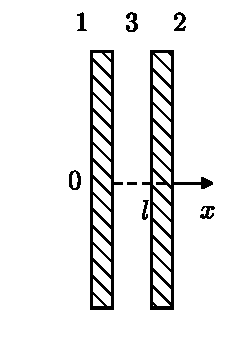
\includegraphics[width=3.0cm]{fig17.pdf}\\[0.3em]
  {\small 图\ 17}
\end{minipage}\par\nopagebreak

\begin{equation}
  \begin{aligned}
    F=\sigma_{xx}(l)= {}& \\
    =\frac{T}{4\pi}\sum_{n=0}^{\infty}{}'\Bigl\{&\mathcal{D}^{E}_{yy}(\zeta_n;l,l)+\mathcal{D}^{E}_{zz}(\zeta_n;l,l)-\mathcal{D}^{E}_{xx}(\zeta_n;l,l)+\\
    &+\mathcal{D}^{H}_{yy}(\zeta_n;l,l)+\mathcal{D}^{H}_{zz}(\zeta_n;l,l)-\mathcal{D}^{H}_{xx}(\zeta_n;l,l)\Bigr\}.
  \end{aligned}
\end{equation}
（本节用字母 n 表示求和下标）.

由于问题在 y 和 z 方向上的均匀性，函数 $\mathcal{D}_{ik}(\zeta_n;\bm{r},\bm{r}')$ 只依赖于差 $y-y'$ 和 $z-z'$［在(80.1)中没写出宗量 $y-y'$ 和 $z-z'$］；$\mathcal{D}_{ik}(\zeta_n,\bm{q};x,x')$ 是按这些变量展开的傅里叶分量.则
\begin{equation}
  \mathcal{D}_{ik}(\zeta_n;\bm{r},\bm{r})=\int\mathcal{D}_{ik}(\zeta_n,\bm{q};x,x)\,\frac{\mathrm{d}^{2}\bm{q}}{(2\pi)^{2}}.
\end{equation}
对函数 $\mathcal{D}_{ik}(\zeta_n,\bm{q};x,x')$，方程(79.8)取如下形式（矢量 $\bm{q}$ 方向沿 y 轴）
\begin{equation*}
  \begin{gathered}
    \Bigl(w^{2}-\frac{\mathrm{d}^{2}}{\mathrm{d}x^{2}}\Bigr)\mathcal{D}_{zz}(x,x')=-4\pi\delta(x-x'),\\
    \Bigl(w^{2}-q^{2}-\frac{\mathrm{d}^{2}}{\mathrm{d}x^{2}}\Bigr)\mathcal{D}_{yy}(x,x')+\mathrm{i}q\,\frac{\mathrm{d}}{\mathrm{d}x}\mathcal{D}_{xy}(x,x')=-4\pi\delta(x-x'),\\
    w^{2}\mathcal{D}_{xy}(x,x')+\mathrm{i}q\,\frac{\mathrm{d}}{\mathrm{d}x}\mathcal{D}_{yy}(x,x')=0,\\
    w^{2}\mathcal{D}_{xx}(x,x')+\mathrm{i}q\,\frac{\mathrm{d}}{\mathrm{d}x}\mathcal{D}_{yx}(x,x')=-4\pi\delta(x-x'),
  \end{gathered}
\end{equation*}
%%p331（印刷页320）
此处 $w=(\varepsilon\zeta_n^{2}+q^{2})^{1/2}$，$\varepsilon=\varepsilon(\mathrm{i}\zeta_n)$，而 $x'$ 起参数作用（分量 $\mathcal{D}_{xz}=\mathcal{D}_{yz}=0$，因为它们的方程是齐次的.）. 解这个方程组归结为只解两个方程：
\begin{equation}
  \Bigl(w^{2}-\frac{\mathrm{d}^{2}}{\mathrm{d}x^{2}}\Bigr)\mathcal{D}_{zz}(x,x')=-4\pi\delta(x-x'),
\end{equation}
\begin{equation}
  \Bigl(w^{2}-\frac{\mathrm{d}^{2}}{\mathrm{d}x^{2}}\Bigr)\mathcal{D}_{yy}(x,x')=-\frac{4\pi w^{2}}{\varepsilon\zeta_n^{2}}\,\delta(x-x'),
\end{equation}
解出之后，$\mathcal{D}_{xy}$ 和 $\mathcal{D}_{xx}$ 由下列方程确定
\begin{equation}
  \begin{aligned}
    \mathcal{D}_{xy}(x,x')&=-\mathrm{i}q/w^{2}\,\frac{\mathrm{d}}{\mathrm{d}x}\mathcal{D}_{yy}(x,x')\\
    \mathcal{D}_{xx}(x,x')&=-\frac{\mathrm{i}q}{w^{2}}\,\frac{\mathrm{d}}{\mathrm{d}x}\mathcal{D}_{yx}(x,x')-\frac{4\pi}{w^{2}}\,\delta(x-x')
  \end{aligned}
\end{equation}
此时应该考虑到，由于(79.5)，$\mathcal{D}_{yx}(\bm{r},\bm{r}')=\mathcal{D}_{xy}(\bm{r}',\bm{r})$，因而
\begin{equation*}
  \mathcal{D}_{yx}(\bm{q};x,x')=\mathcal{D}_{xy}(-\bm{q};x',x).
\end{equation*}
与电磁场强度切线分量连续性相对应的边界条件，归结为 $\mathcal{D}^{E}_{yk},\allowbreak\mathcal{D}^{E}_{zk},\allowbreak\mathcal{D}^{H}_{yk},\allowbreak\mathcal{D}^{H}_{zk}$ 的连续性或者 $\mathcal{D}_{yk},\allowbreak\mathcal{D}_{zk},\allowbreak\mathrm{rot}_{yl}\mathcal{D}_{lk},\allowbreak\mathrm{rot}_{zl}\mathcal{D}_{lk}$ 量的连续性.

利用(81.5)的第一等式，得出
\begin{equation}
  \mathcal{D}_{zz},\quad \frac{\mathrm{d}}{\mathrm{d}x}\mathcal{D}_{zz},\quad \mathcal{D}_{yy},\quad \frac{\varepsilon}{w^{2}}\,\frac{\mathrm{d}}{\mathrm{d}x}\mathcal{D}_{yy},
\end{equation}
在分界面上必须连续.

因为考虑到只在间隙区域计算应力张量.所以立即认为 $0<x'<l$. 在 $0<x<l$ 区域，函数 $\mathcal{D}_{yy}$ 和 $\mathcal{D}_{zz}$ 由 $\varepsilon=1$，$w=w_3=(\zeta_n^{2}+q^{2})^{1/2}$ 的方程(81.3—81.4)确定.在区域 $1\,(x<0)$ 和区域 $2\,(x>0)$，这些函数仍然满足将 $\varepsilon$，w 取做 $\varepsilon_1,w_1$ 和 $\varepsilon_2,w_2$ 的那两个方程，此时方程的右侧均为零（因为在此 $x\neq x'$）.

根据(80.17)，所需要的减除，应归结为从间隙区域中的所有函数 $\mathcal{D}_{ik}$ 减去这些函数在 $\varepsilon_1=\varepsilon_2=1$ 之值.从而，特别是，可以略去(81.5)的第二等式右边的第二项，于是在间隙区域
\begin{equation}
  \mathcal{D}_{xy}=-\frac{\mathrm{i}q}{w_3^{2}}\,\frac{\partial}{\partial x}\mathcal{D}_{yy},\qquad \mathcal{D}_{xx}=-\frac{\mathrm{i}q}{w_3^{2}}\,\frac{\mathrm{d}}{\mathrm{d}x}\mathcal{D}_{yx}.
\end{equation}
%%p332（印刷页321）
在解方程之前，还要做一注记.方程(81.3—81.4)的一般解的形式是 $f^{-}(x-x')+f^{+}(x+x')$.利用方程(81.3—81.4)，(81.7)和函数 $\mathcal{D}^{E}_{ik}$ 及 $\mathcal{D}^{H}_{ik}$ 的定义，可以证明：与 $x+x'$ 之和有关的那部分格林函数 $\mathcal{D}^{E}_{ik}$ 和 $\mathcal{D}^{H}_{ik}$，对于力的表达式(81.1)没有任何贡献.在此我们不讲这个问题，因为这个结果从物理考虑中早已看出：如在形为 $f^{+}(x+x')$ 的解中取 $x=x'$，在间隙内我们就会得到与坐标有关的动量流——这与动量守恒定律相矛盾.因此，今后在结果中我们只引用与 $x+x'$ 无关的那部分格林函数 $\mathcal{D}_{ik}$ 的表达式.

现在我们来求函数 $\mathcal{D}_{zz}$.它满足方程：
\begin{equation}
  \left.\begin{aligned}
    \Bigl(w_1^{2}-\frac{\mathrm{d}^{2}}{\mathrm{d}x^{2}}\Bigr)\mathcal{D}_{zz}(x,x')&=0, & x<0,\\
    \Bigl(w_2^{2}-\frac{\mathrm{d}^{2}}{\mathrm{d}x^{2}}\Bigr)\mathcal{D}_{zz}(x,x')&=0, & x>l,\\
    \Bigl(w_3^{2}-\frac{\mathrm{d}^{2}}{\mathrm{d}x^{2}}\Bigr)\mathcal{D}_{zz}(x,x')&=-4\pi\delta(x-x'), & 0<x<l.
  \end{aligned}\right\}
\end{equation}
由此得到
\begin{equation*}
  \begin{gathered}
    \mathcal{D}_{zz}=A\mathrm{e}^{w_1 x},\quad x<0,\qquad \mathcal{D}_{zz}=B\mathrm{e}^{-w_2 x},\quad x>l.\\
    \mathcal{D}_{zz}=C_1\mathrm{e}^{w_3 x}+C_2\mathrm{e}^{-w_3 x}-\frac{2\pi}{w_3}\,\mathrm{e}^{-w_3|x-x'|},\quad 0<x<l.
  \end{gathered}
\end{equation*}
在最后表达式中已考虑到：由于(81.8)第三方程中的微商 $\mathrm{d}\mathcal{D}_{zz}/\mathrm{d}x$ 在 $x=x'$ 处有等于 $4\pi$ 的跃变. 因 $\mathcal{D}_{zz}$ 和 $\mathrm{d}\mathcal{D}_{zz}/\mathrm{d}x$ 需要连续的边界条件来确定 $A,B,C_1,C_2$（$x'$ 的函数），之后我们得到
\begin{equation*}
  \mathcal{D}_{zz}=\frac{4\pi}{w_3\Delta}\,\mathrm{cosh}\,w_3(x-x')-\frac{2\pi}{w_3}\,\mathrm{e}^{-w_3|x-x'|},\quad 0<x<l.
\end{equation*}
此处
\begin{equation*}
  \Delta=1-\mathrm{e}^{2w_3 l}\,\frac{(w_1+w_3)(w_2+w_3)}{(w_1-w_3)(w_2-w_3)}.
\end{equation*}
减去 $\mathcal{D}_{zz}$ 在 $w_1=w_2=w_3$（此时 $1/\Delta=0$）的值. 最后我们有
\begin{equation*}
  \mathcal{D}_{zz}=\frac{4\pi}{w_3\Delta}\,\mathrm{cosh}\,w_3(x-x').
\end{equation*}
类似地解 $\mathcal{D}_{yy}$ 的方程，我们得到（减除之后）
\begin{equation*}
  \mathcal{D}_{yy}=\frac{4\pi w_3}{\zeta_n^{2}\Delta_1}\,\mathrm{cosh}\,w_3(x-x'),
\end{equation*}
\begin{equation*}
  \Delta_1=1-\mathrm{e}^{2w_3 l}\,\frac{(\varepsilon_1 w_3+w_1)(\varepsilon_2 w_3+w_2)}{(\varepsilon_1 w_3-w_1)(\varepsilon_2 w_3-w_2)},
\end{equation*}
并利用(81.7)得
\begin{equation*}
  \begin{aligned}
    \mathcal{D}_{xy}=\mathcal{D}_{yx}&=-\frac{4\pi\,\mathrm{i}q}{\zeta_n^{2}\Delta_1}\,\mathrm{sinh}\,w_3(x-x'),\\
    \mathcal{D}_{xx}&=-\frac{4\pi q^{2}}{\zeta_n^{2}w_3\Delta_1}\,\mathrm{cosh}\,w_3(x-x').
  \end{aligned}
\end{equation*}
%%p333（印刷页322）
现在算出函数 $\mathcal{D}^{E}_{ik}$ 和 $\mathcal{D}^{H}_{ik}$，根据(81.2)，将他们变换后，代入(81.1)，我们得到
\begin{equation*}
  F(l)=-\frac{T}{2\pi}\sum_{n=0}^{\infty}{}'\int_{0}^{\infty}w_3\biggl(\frac{1}{\Delta}+\frac{1}{\Delta_1}\biggr)q\,\mathrm{d}q.
\end{equation*}
最后，根据 $q=\zeta_n\sqrt{p^{2}-1}$，变换到新的积分变量 $p$，并返回通常单位，我们得到作用力 $\bm{F}$ 的最终表达式，即作用于被宽度为 l 的间隙隔开的两物体中每一物体的单位面积上的力：
\begin{equation}
  \begin{aligned}
    F(l)=\frac{T}{\pi c^{3}}\sum_{n=0}^{\infty}{}'\zeta_n^{3}\int_{1}^{\infty}p^{2}\biggl\{\biggl[\frac{(s_1+p)(s_2+p)}{(s_1-p)(s_2-p)}\,\mathrm{exp}\biggl(\frac{2p\zeta_n}{c}\,l\biggr)-1\biggr]^{-1}+\\
    +\biggl[\frac{(s_1+p\varepsilon_1)(s_2-p\varepsilon_2)}{(s_1-p\varepsilon_1)(s_2-p\varepsilon_2)}\,\mathrm{exp}\biggl(\frac{2p\zeta_n}{c}\,l\biggr)-1\biggr]^{-1}\biggr\}\mathrm{d}p,
  \end{aligned}
\end{equation}
此处 $s_1=\sqrt{\varepsilon_1-1+p^{2}}$，$s_2=\sqrt{\varepsilon_2-1+p^{2}}$，$\zeta_n=2\pi nT/\hbar$，$\varepsilon_1,\varepsilon_2$ 是虚数频率 $\omega=\mathrm{i}\zeta_n$ 的函数；联想到 $\varepsilon(\mathrm{i}\zeta)$ 是正的实值，它从 $\zeta=0$ 时自己的静电值 $\varepsilon_0$ 单调减少到 $\zeta=\infty$ 时的1\footnote{推导公式(81.9)时，假设两个物体是各向同性的.因此，它对晶体的应用与可以忽略电容率的各向异性有关.虽然在大多数情况下这是完全允许的，但应注意到，一般来说，物体的各向异性，还导致特殊效应——出现使物体趋于相互转动的力矩.}.F 的正值对应于物体的吸引力.(81.9)的每一求和项的被积式都是正的，并且对每一给定 p 和 $\zeta_n$ 的值，都随 l 的增长而单调减少\footnote{只要指出，对于 $s=(\varepsilon-1+p^{2})^{1/2}$（此处 $p\geqslant 1$），当 $\varepsilon>1$ 时，有不等式 $\varepsilon p>s>p$，就容易相信这一点.}，由此得出，$F>0$，$\mathrm{d}F/\mathrm{d}l<0$，也就是由空隙分开的物体，以随距离增加而单调减少的力吸引着.

一般公式(81.9)是很复杂的.然而，通常由于温度对相互作用力的影响完全不重要，故此公式可以大大简化\footnote{在讲到温度影响时，我们不考虑电容率本身与温度有关的方面.}.问题是，由于在(81.9)中的被积式中存在指数函数，故在求和中只有 $\zeta_n\sim c/l$ 或 $n\sim c\hbar/lT$ 的项起主要作用.这样一来，在 $lT/c\hbar\ll 1$ 的情况下，大 n 值才是重要的，因此在(81.9)中，可以从求和过渡到按 $\mathrm{d}n=\hbar\,\mathrm{d}\zeta/2\pi T$ 的积分.此时，温度从公式中消失，从而我们得到如下结果：
\begin{equation}
  \begin{aligned}
    F(l)=\frac{\hbar}{2\pi^{2}c^{3}}\int_{0}^{\infty}\!\!\int_{1}^{\infty}p^{2}\zeta^{3}\biggl\{\biggl[\frac{(s_1+p)(s_2+p)}{(s_1-p)(s_2-p)}\,\mathrm{exp}\biggl(\frac{2p\zeta}{c}\,l\biggr)-1\biggr]^{-1}+\\
    +\biggl[\frac{(s_1+p\varepsilon_1)(s_2+p\varepsilon_2)}{(s_1-p\varepsilon_1)(s_2-p\varepsilon_2)}\,\mathrm{exp}\biggl(\frac{2p\zeta}{c}\,l\biggr)-1\biggr]^{-1}\biggr\}\mathrm{d}p\,\mathrm{d}\zeta.
  \end{aligned}
\end{equation}
%%p334（印刷页323）
据上所述，此公式适用于 $l\ll c\hbar/T$ 的距离；在室温下此式给出的距离甚至达到 $\sim 10^{-4}\,\mathrm{cm}$.公式(81.10)在两种极限情况下还可进一步大大简化.

\section{固体间相互作用的分子力·极限情况}

首先我们讲述"小"距离的极限情况，这个"小"距离，意味着它比给定物体的吸收谱的特征波长 $\lambda_0$ 小.至于讲到凝聚体的温度，在任何情况下它都小于在此起作用的 $\hbar\omega_0$（例如，在可见谱段），因此关于 $a$ 的不等式显然是满足的.

由于被积式的分母有指数函数因子，在按 $\mathrm{d}p$ 积分时重要的是 $p\zeta l/c\sim 1$ 的区域.此时，$p\gg 1$，所以在确定积分的主要项时可设 $s_1\approx s_2\approx p$. 在此近似下，(81.10)花括号中的第一项变为零.第二项在引入 $x=2p\zeta l/c$ 的积分变量后给出
\begin{equation}
  F(l)=\frac{\hbar}{16\pi^{2}l^{3}}\int_{0}^{\infty}\!\!\int_{0}^{\infty}x^{2}\biggl[\frac{(\varepsilon_1+1)(\varepsilon_2+1)}{(\varepsilon_1-1)(\varepsilon_2-1)}\,\mathrm{e}^{x}-1\biggr]^{-1}\mathrm{d}x\,\mathrm{d}\zeta
\end{equation}
（在此近似下 dx 积分的下限用零来代替）\footnote{当 $a$ 由 $\infty$ 变到 1 时，下述积分
\begin{equation*}
  \frac{a}{2}\int_{0}^{\infty}\frac{x^{2}\,\mathrm{d}x}{a\mathrm{e}^{x}-1}
\end{equation*}
的变化不大：由 1 到 1.2. 因此实际上可以足够精确地将公式(82.1)写为下列形式
\begin{equation*}
  F=\frac{\hbar\bar{\omega}}{8\pi^{2}l^{3}},\qquad
  \bar{\omega}=\int_{0}^{\infty}\frac{\bigl[\varepsilon_1(\mathrm{i}\zeta)-1\bigr]\bigl[\varepsilon_2(\mathrm{i}\zeta)-1\bigr]}{\bigl[\varepsilon_1(\mathrm{i}\zeta)+1\bigr]\bigl[\varepsilon_2(\mathrm{i}\zeta)+1\bigr]}\,\mathrm{d}\zeta,
\end{equation*}
量 $\bar{\omega}$ 对于两个物体的吸收谱来说起着某种特征频率的作用.}.

在此情况下力与距离的三次方成反比，不过，我们期望，这对应于两个原子间范德瓦耳斯力通常的规律（见324页的底注）. 函数 $\varepsilon(\mathrm{i}\zeta)-1$ 随 $\zeta$ 的增加而单调减少并趋于零.因此，从某个 $\zeta\sim\zeta_0$ 开始，$\zeta$ 值在积分中就不再提供主要的贡献；l 小的条件表明必须有 $l\ll c/\zeta_0$.

我们证明：如何能由宏观公式(82.1)过渡到真空中的个别原子之间的相互作用.为此，我们形式地假设两个物体都足够稀薄.从宏观的观点来看，这意味着它们的电容率接近于1，也就是差 $\varepsilon_1-1$ 和 $\varepsilon_2-1$ 都小.则从(82.1)得出所需精度的公式
\begin{equation*}
  \begin{aligned}
    F&=\frac{\hbar}{64\pi^{2}l^{3}}\int_{0}^{\infty}\!\!\int_{0}^{\infty}x^{2}\,\mathrm{e}^{-x}(\varepsilon_1-1)(\varepsilon_2-1)\,\mathrm{d}x\,\mathrm{d}\zeta=\\
    &=\frac{\hbar}{32\pi^{2}l^{3}}\int_{0}^{\infty}\bigl[\varepsilon_1(\mathrm{i}\zeta)-1\bigr]\bigl[\varepsilon_2(\mathrm{i}\zeta)-1\bigr]\,\mathrm{d}\zeta.
  \end{aligned}
\end{equation*}
在实轴 $\omega$ 上将 $\varepsilon(\mathrm{i}\zeta)$ 通过 $\mathrm{Im}\,\varepsilon(\omega)$ 表达出来，根据(80.18)得
\begin{equation}
  \begin{aligned}
    F&=\frac{\hbar}{8\pi^{4}l^{3}}\int\!\!\!\int\!\!\!\int_{0}^{\infty}\frac{\omega_1\omega_2\,\mathrm{Im}\,\varepsilon_1(\omega_1)\,\mathrm{Im}\,\varepsilon_2(\omega_2)}{(\omega_1^{2}+\zeta^{2})(\omega_2^{2}+\zeta^{2})}\,\mathrm{d}\zeta\,\mathrm{d}\omega_1\,\mathrm{d}\omega_2=\\
    &=\frac{\hbar}{16\pi^{3}l^{3}}\int\!\!\!\int_{0}^{\infty}\frac{\mathrm{Im}\,\varepsilon_1(\omega_1)\,\mathrm{Im}\,\varepsilon_2(\omega_2)}{\omega_1+\omega_2}\,\mathrm{d}\omega_1\,\mathrm{d}\omega_2.
  \end{aligned}
\end{equation}
%%p335（印刷页324）
这个力相当于原子以如下的能量相互作用着，
\begin{equation}
  U(\bm{r})=-\frac{3\hbar}{8\pi^{4}n_1 n_2 r^{6}}\int\!\!\!\int\frac{\mathrm{Im}\,\varepsilon_1(\omega_1)\,\mathrm{Im}\,\varepsilon_2(\omega_2)}{\omega_1+\omega_2}\,\mathrm{d}\omega_1\,\mathrm{d}\omega_2.
\end{equation}
此处 r 是原子间的距离；$n_1,n_2$ 是两个物体的原子数密度\footnote{如果原子 1 和原子 2 的相互作用势能是 $U(r)=-ar^{-6}$，那么被宽为 $l$ 的空隙所分开的两个半空间中，所有原子的成对相互作用总能量等于 $U_{\text{隙}}=-a\pi n_1 n_2/(12l^{2})$. 力是 $F=\mathrm{d}U_{\text{隙}}/\mathrm{d}l=a\pi n_1 n_2/(6l^{3})$. 这就是公式(82.2)和(82.3)的对应关系.}.这个公式与普通微扰论应用于双原子偶极相互作用而得出的著名的量子力学伦敦公式一致（见第三卷§89，习题）.在对比中应考虑到 $\varepsilon(\omega)$ 的虚部与"振子力"的谱密度 $f(\omega)$ 有如下的关系
\begin{equation*}
  \omega\,\mathrm{Im}\,\varepsilon(\omega)=\frac{2\pi^{2}e^{2}}{m}\,n f(\omega)
\end{equation*}
（e,m 是电子的电荷和质量；见第八卷§62）；振子力用已知的方法通过原子偶极矩的矩阵元的平方来表述［见第三卷(149.10)］.

我们来研究相反的"大"距离情况：$l\gg\lambda_0$. 然而，此时我们认为距离仍然不致大到打破不等式 $lT/\hbar c\ll 1$ 的程度.

在公式(81.10)中重新引入新的积分变量 $x=2pl\zeta/c$，但作为第二个变量的不是 $\zeta$，而是 $p$.则 $\varepsilon_1$ 和 $\varepsilon_2$ 是宗量 $\mathrm{i}\zeta=\mathrm{i}xc/2pl$ 的函数.但由于在被积式的分母中存在 $\mathrm{e}^{x}$，在按 dx 的积分中，有意义的是 $x\sim 1$ 的各值，因为 $p\geqslant 1$，则在大值 l 情况下，函数 $\varepsilon$ 的宗量在变量的一切重要区域都接近于零.与此相应，我们可以简单地将 $\varepsilon_1,\varepsilon_2$ 以它在 $\zeta=0$ 的值，也就是用静电电容率 $\varepsilon_{10},\varepsilon_{20}$ 来代替.这样一来，最后
\begin{equation}
  \begin{aligned}
    F=\frac{\hbar c}{32\pi^{2}l^{4}}\int_{0}^{\infty}\!\!\int_{1}^{\infty}\frac{x^{3}}{p^{2}}\biggl\{&\biggl[\frac{(s_{10}+p)(s_{20}+p)}{(s_{10}-p)(s_{20}-p)}\,\mathrm{e}^{x}-1\biggr]^{-1}+\\
    +&\biggl[\frac{(s_{10}+p\varepsilon_{10})(s_{20}+p\varepsilon_{20})}{(s_{10}-p\varepsilon_{10})(s_{20}-p\varepsilon_{20})}\,\mathrm{e}^{x}-1\biggr]^{-1}\biggr\}\mathrm{d}p\,\mathrm{d}x,\\
    &s_{10}=\sqrt{\varepsilon_{10}-1+p^{2}},\qquad s_{20}=\sqrt{\varepsilon_{20}-1+p^{2}}.
  \end{aligned}
\end{equation}
力随距离（如 $l^{-4}$）增加而减少的规律，在此情况下对应于两原子间范德瓦耳斯力因计及推迟而减少的规律（见下面）.

%%p336（印刷页325）
当两物体是金属时，公式(82.4)归之为十分简单的表达式.对于金属，当 $\zeta\to 0$ 时，函数 $\varepsilon(\mathrm{i}\zeta)\to\infty$；因此，对于金属应认为 $\varepsilon_0=\infty$. 取 $\varepsilon_{10}=\varepsilon_{20}=\infty$，我们得到
\begin{equation}
  F=\frac{\hbar c}{16\pi^{2}l^{4}}\int_{0}^{\infty}\!\!\int_{1}^{\infty}\frac{x^{3}\,\mathrm{d}p\,\mathrm{d}x}{p^{2}(\mathrm{e}^{x}-1)}=\frac{\pi^{2}\hbar c}{240\,l^{4}}
\end{equation}
（H.~B.~G.~Casimir，1948）. 这个力根本与金属的种类无关［这性质在小距离处不出现，此处相互作用力不仅在 $\zeta=0$，而且在所有 $\zeta$ 值的情况下都依赖于函数 $\varepsilon(\mathrm{i}\zeta)$ 的行为］.

图 18 是函数 $\phi_{\mathrm{II}}(\varepsilon_0)$ 的图，此函数确定两个相同电介质（$\varepsilon_{10}=\varepsilon_{20}=\varepsilon_0$）之间的引力.公式(82.4)的形式如下
\begin{equation}
  F=\frac{\pi^{2}\hbar c}{240\,l^{4}}\biggl(\frac{\varepsilon_0-1}{\varepsilon_0+1}\biggr)^{2}\phi_{\mathrm{II}}(\varepsilon_0)
\end{equation}

\par\nopagebreak\noindent\begin{minipage}{\linewidth}\centering
  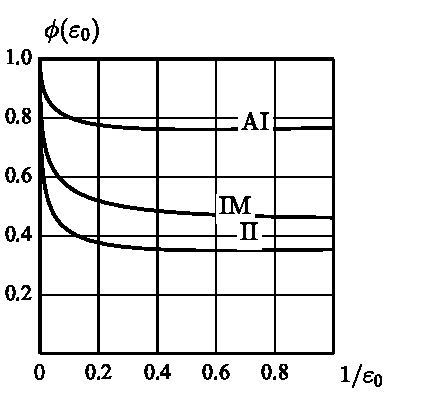
\includegraphics[width=7.5cm]{fig18.pdf}\\[0.3em]
  {\small 图\ 18}
\end{minipage}\par\nopagebreak

在这个图上还给出函数 $\phi_{\mathrm{IM}}$ 的图.此函数根据下列公式\footnote{当 $\varepsilon_0\to 1$ 时，函数 $\phi_{\mathrm{II}}$ 和 $\phi_{\mathrm{IM}}$ 值分别趋近于 0.35 和 0.46. 这与极限规律(82.8)以及本节习题(1)式相对应. 当 $\varepsilon_0\to\infty$ 时，两个函数趋近于与公式(82.5)相应的数值 1.}确定电介质和金属（$\varepsilon_{10}=\varepsilon_0$，$\varepsilon_{20}=\infty$）之间的引力.
\begin{equation}
  F=\frac{\pi^{2}\hbar c}{240\,l^{4}}\,\frac{\varepsilon_0-1}{\varepsilon_0+1}\,\phi_{\mathrm{IM}}(\varepsilon_0).
\end{equation}
类似于以前(82.1)所做的，我们在(84.4)中，过渡到个别原子间的相互作用. 在 $\varepsilon_0-1$ 很小的情况下，我们有
\begin{equation*}
  s_0-p\approx\frac{\varepsilon_0-1}{2p},\qquad s_0-p\varepsilon_0\approx(\varepsilon_0-1)\biggl(-p+\frac{1}{2p}\biggr),
\end{equation*}
%%p337（印刷页326）
积分(82.4)取下列形式
\begin{equation*}
  F=\frac{\hbar c}{32\pi^{2}l^{4}}(\varepsilon_{10}-1)(\varepsilon_{20}-1)\int_{0}^{\infty}x^{3}\,\mathrm{e}^{-x}\,\mathrm{d}x\int_{1}^{\infty}\frac{1-2p^{2}+2p^{4}}{8p^{6}}\,\mathrm{d}p,
\end{equation*}
由此得
\begin{equation}
  F=\frac{\hbar c}{l^{4}}\,\frac{23}{640\pi^{2}}(\varepsilon_{10}-1)(\varepsilon_{20}-1).
\end{equation}
这个力相当于两个原子以能量
\begin{equation}
  U(r)=-\frac{23\hbar c}{4\pi r^{7}}\,\alpha_1\alpha_2
\end{equation}
相互作用，此处 $\alpha_1,\alpha_2$ 是原子静极化系数（$\varepsilon_0=1+4\pi n\alpha$）.公式(82.9)和量子电动力学在足够大的距离上（此时推迟效应已甚为重要），对两个原子间引力的计算结果相一致（见第四卷§85）.

最后，我们研究使不等式 $lT/\hbar c\gg 1$ 成立的大距离，这与可能忽视温度影响的要求相反.在此情况下(81.9)的所有求和项中只需保留第一项.然而，其中不可一开始就取 $n=0$，因为这要产生不确定性：（因子 $\zeta_n^{3}$ 变为零，但对 dp 积分是发散的）. 如果开头就用新的积分变量 $x=2p\zeta_n l/c$ 来代替 p，这个困难就可避免（从而因子 $\zeta_n^{3}$ 消失）. 然后取 $\zeta_n=0$，我们得到
\begin{equation}
  F=\frac{T}{16\pi l^{3}}\int_{0}^{\infty}x^{2}\biggl[\frac{(\varepsilon_{10}+1)(\varepsilon_{20}+1)}{(\varepsilon_{10}-1)(\varepsilon_{20}-1)}\,\mathrm{e}^{x}-1\biggr]^{-1}\mathrm{d}x
\end{equation}
这样一来，在足够大的距离上，引力减小得慢了，又重新出现规律 $l^{-3}$. 但系数与温度有关［(81.9)求和中的一切后续项都随 l 增大而作指数衰减］. 条件 $lT/\hbar c\gg 1$ 本质上是经典性的条件（$\hbar\omega\ll T$，此处 $\omega\sim c/l$）. 因此，自然地，(82.10)中不包含 $\hbar$\footnote{§81，§82 得到的公式，能够推广到固体间隙内充以液体的情况，以及在固体表面上有薄液膜的情况. 见 И.\,Е.\,Дзялошинский, Е.\,М.\,Лифшиц, Л.\,П.\,Питаевский, УФН, 78, 381, 1961 (Soviet physics Uspekhi 4, 153, 1961; Advances in Phys., V.~10, P.~165, 1961.).}

\begin{xiti}

试求原子与金属壁在"大"距离上的相互作用规律.

{\heiti 解：}单个原子与凝聚体的相互作用，只要将其中一个物体（设为物体 2）看做是稀薄的介质就可得到.如认为 $\varepsilon_{20}-1$ 很小，并取 $\varepsilon_{10}=\infty$，从(82.4)得到
\begin{equation}\tag{1}
  F=\frac{\hbar c(\varepsilon_{20}-1)}{32\pi^{2}l^{4}}\int_{0}^{\infty}x^{3}\,\mathrm{e}^{-x}\,\mathrm{d}x\int_{1}^{\infty}\frac{\mathrm{d}p}{2p^{2}}=\frac{3\hbar c(\varepsilon_{20}-1)}{32\pi^{2}l^{4}}.
\end{equation}
%%p338（印刷页327）
如果原子与壁之间的相互作用能 $U=-aL^{-4}$（L 是原子和壁之间的距离），则在靠壁空隙 l 的半空间内，原子之间的相互作用能为 $U_{\text{隙}}=-an/3l^{3}$，而力 $F=\mathrm{d}U_{\text{隙}}/\mathrm{d}l=an/l^{4}$，因此，得到的 F 值对应于单个原子与壁以如下能量相互吸引：
\begin{equation}\tag{2}
  U(L)=-3\alpha_2\hbar c/8\pi L^{4}
\end{equation}
（H.~B.~G.~Casimir, D.~Polder, 1948）.

同理，对于原子和介电壁的相互作用，可得下列结果
\begin{equation*}
  U(L)=-\frac{3\hbar c\,\alpha_2}{8\pi L^{4}}\times\frac{(\varepsilon_{10}-1)}{(\varepsilon_{10}+1)}\,\phi_{\mathrm{AI}}(\varepsilon_{10})
\end{equation*}
其函数 $\phi_{\mathrm{AI}}$ 如图 18. 当 $\varepsilon_{10}\to 1$ 时，此函数趋近于与公式(82.8)相应的值 $23/30=0.77$.

\end{xiti}

\section{液体中关联函数的渐近行为}

长波电磁涨落也使均匀液体密度涨落的关联函数具有某些特殊性质.

我们记得（见第五卷§116），关联函数 $\nu(r)$ 定义于：在空间两点粒子数密度 n 的涨落乘积的平均值为
\begin{equation}
  \begin{gathered}
    \bigl\langle\delta n(\bm{r}_1)\,\delta n(\bm{r}_2)\bigr\rangle=\bar{n}\,\delta(\bm{r})+\bar{n}\,\nu(\bm{r}),\\
    \bm{r}=\bm{r}_1-\bm{r}_2.
  \end{gathered}
\end{equation}
关联函数与粒子间的相互作用有关，该函数在大距离上的渐近行为，由这个作用的远程范德瓦尔斯部分所决定.因此 $\nu(r)$ 和范德瓦尔斯力一样，随距离增加而按幂的规律减小(J.~Enderby, T.~Gaskell, N.~H.~March, 1965).

当然这也反映在关联函数傅里叶分量 $\nu(\bm{k})\equiv\nu(\bm{k})$ 的性质上.如果液体粒子间的相互作用只是作用半径数量级为原子线度 a 的力，那么函数 $\nu(r)$ 将随距离按指数为 r/a 的指数函数规律减少\footnote{这里所讲的情况是液体处在温度 $T\sim\Theta$（$\Theta\sim\hbar u/a$ 是液体的"德拜温度"）并且远离临界点. 在临界点附近，关联半径是无限增长的（见第五卷§152，§153）. 在 $T\ll\Theta$ 的低温下，关联半径也能增长到 $\hbar u/T$ 的数量级（见下面的§87）.}.在傅里叶分量的术语中，这意味着，$\nu(\bm{k})$ 是 ka 的正则函数，它在 $ka\ll 1$ 的情况下是按 ka 的偶次幂展开的.远程力在 $k\sim 1/\lambda_0$（而不是 $k\sim 1/a$）的区域内，在 $\nu(\bm{k})$ 中已经有明显变化的项［以 $\nu_1(k)$ 表示］出现，此处 $\lambda_0$ 是液体谱中的特征波长（$\lambda_0\gg a$）.在 $ka\ll 1$ 的区域内，参数 $k\lambda_0$ 可小可大；函数 $\nu_1(k)$ 在这区域内具有奇异性质.

为了计算关联函数，我们利用此函数与物体自由能对其密度的二阶变分微商的关系.按定义，这个微商是自由能的变化与密度涨落（当温度给定时）的关系式中的 $\varphi$：
\begin{equation}
  \delta F=\frac{1}{2}\int\varphi\bigl(|\bm{r}_1-\bm{r}_2|\bigr)\delta n(\bm{r}_1)\,\delta n(\bm{r}_2)\,\mathrm{d}^{3}x_1\,\mathrm{d}^{3}x_2,
\end{equation}
%%p339（印刷页328）
这个函数的傅里叶分量 $\varphi(\bm{k})\equiv\varphi(\bm{k})$ 与待求函数 $\nu(\bm{k})$ 的关系为
\begin{equation}
  \nu(\bm{k})=\frac{T}{\bar{n}\,\varphi(\bm{k})}-1
\end{equation}
［见第五卷(116.14)］.我们强调指出，这个公式假设涨落是经典的，它要求 $\hbar\omega\ll T$. 此处 $\omega$ 是波矢为 $\bm{k}$ 的振动频率. 取 $\omega\sim ku$（此处 u 是液体中的声速），我们得到条件
\begin{equation}
  \hbar ku\ll T,
\end{equation}
这与距离 $r\gg\hbar u/T$ 相对应.

与短程作用力有关的函数 $\varphi(\bm{k})$ 的"正则"部分，是按 k 的幂展开的第一项（当 $ka\ll 1$）并用 b 来表示它，可写出
\begin{equation}
  \varphi(\bm{k})\approx b+\varphi_1(\bm{k}),
\end{equation}
此处 $\varphi_1(\bm{k})$ 是我们感兴趣的函数 $\varphi(\bm{k})$ 的"奇异"部分\footnote{常数 $b$ 通过液体的热力学量以 $b=\dfrac{1}{\bar{n}}\biggl(\dfrac{\partial P}{\partial\bar{n}}\biggr)_{T}$ 来表示（见第五卷§152）.}.由于范德瓦尔斯力比较弱，$\varphi_1(\bm{k})\ll b$，因此，将(83.5)代入(83.3)，结果可表为如下形式
\begin{equation}
  \nu(\bm{k})=\frac{T}{\bar{n}b}-1-\frac{T}{\bar{n}b^{2}}\,\varphi_1(\bm{k}).
\end{equation}
因为 $\nu(\bm{k})$ 跟 $\varphi_1(\bm{k})$ 是线性关系，所以函数 $\nu(r)$ 在大距离上就是
\begin{equation}
  \nu(r)=-\frac{T}{\bar{n}b^{2}}\,\varphi_1(r).
\end{equation}
(83.6)中的第一项（不依赖于 k）对应于短程作用力（忽视其作用半径时），是形如 $\mathrm{const}\cdot\delta(\bm{r})$ 的坐标函数.

我们从自由能变分的公式(80.11)出发，来确定 $\varphi_1(r)$. 在公式中写出
\begin{equation}
  \delta\varepsilon(\mathrm{i}\zeta,\bm{r})=\frac{\partial\varepsilon(\mathrm{i}\zeta)}{\partial\bar{n}}\,\delta n(\bm{r}).
\end{equation}
我们看出，表达式
\begin{equation*}
  -\frac{T}{4\pi\hbar c^{2}}\sum_{s=0}^{\infty}{}'\zeta_s^{2}\,\mathcal{D}_{ii}(\zeta_s;\bm{r},\bm{r})\,\frac{\partial\varepsilon(\mathrm{i}\zeta_s)}{\partial\bar{n}}
\end{equation*}
乃是自由能对密度的一阶变分微商. 同样，对于二阶微商，应当变分这个公式，亦即求\footnote{只有对函数 $\mathcal{D}_{ii}$ 变分. 变分函数 $\varepsilon$ 在 $\varphi(\bm{r})$ 中将出现与远程作用力无关的，形如 $\mathrm{const}\cdot\delta(\bm{r})$ 的项.}
\begin{equation}
  -\frac{T}{4\pi\hbar c^{2}}\sum_{s=0}^{\infty}{}'\zeta_s^{2}\,\delta\mathcal{D}_{ii}(\zeta_s;\bm{r},\bm{r})\,\frac{\partial\varepsilon(\mathrm{i}\zeta_s)}{\partial\bar{n}}.
\end{equation}
%%p340（印刷页329）
$\mathcal{D}$ 函数本身满足方程(79.8)：
\begin{equation}
  \Bigl[\frac{\partial^{2}}{\partial x_i\,\partial x_l}-\delta_{il}\Delta+\frac{\zeta_s^{2}}{c^{2}}\,\bm{\varepsilon}(\mathrm{i}\zeta_s,\bm{r})\,\delta_{il}\Bigr]\mathcal{D}_{lk}(\zeta_s;\bm{r},\bm{r}')=-4\pi\hbar\,\delta_{ik}\,\delta(\bm{r}-\bm{r}'),
\end{equation}
而它的变分给出 $\mathcal{D}$ 函数的变分方程：
\begin{equation}
  \Bigl[\frac{\partial^{2}}{\partial x_i\,\partial x_l}-\delta_{il}\Delta+\frac{\zeta_s^{2}}{c^{2}}\,\varepsilon(\mathrm{i}\zeta_s)\,\delta_{il}\Bigr]\delta\mathcal{D}_{lk}(\zeta_s,\bm{r},\bm{r}')=-\frac{\zeta_s^{2}}{c^{2}}\,\delta\varepsilon(\mathrm{i}\zeta_s,\bm{r})\,\mathcal{D}_{ik}(\zeta_s;\bm{r},\bm{r}').
\end{equation}
只要根据(83.10)，注意到"非微扰"格林函数 $\mathcal{D}_{ik}$ 就是这个方程的格林函数，方程(83.11)的解便可立即写出；因此，
\begin{equation*}
  \delta\mathcal{D}_{ik}(\zeta_s;\bm{r},\bm{r}')=\frac{\zeta_s^{2}}{4\pi\hbar c^{2}}\int\delta\varepsilon(\mathrm{i}\zeta_s,\bm{r}'')\,\mathcal{D}_{lk}(\zeta_s;\bm{r}'',\bm{r}')\,\mathcal{D}_{li}(\zeta_s;\bm{r}'',\bm{r})\,\mathrm{d}^{3}x''.
\end{equation*}
［在此也用了 $\mathcal{D}_{il}(\bm{r},\bm{r}'')=\mathcal{D}_{li}(\bm{r}'',\bm{r})$］.最后，将(83.8)代入此式，然后与(83.9)一起，我们得到二阶变分微商
\begin{equation}
  \varphi_1(r)=-\frac{T}{(4\pi\hbar c^{2})^{2}}\sum_{s=0}^{\infty}{}'\zeta_s^{4}\biggl[\frac{\partial\varepsilon(\mathrm{i}\zeta_s)}{\partial\bar{n}}\biggr]^{2}\mathcal{D}^{2}_{lm}(\zeta_s;\bm{r}_1,\bm{r}_2).
\end{equation}
（$r=|\bm{r}_1-\bm{r}_2|$）. 当 $r\gg\hbar u/T$ 时这个公式连同(83.7)给出待求的关联函数 $\nu(r)$ 的普遍表达式(М.\,П.\,Кемоклидзе，Л.\,М.\,Питаевский，1970).

前面所取波矢量的条件(83.4)等价于距离的条件 $r\gg\hbar u/T$. 与这个条件同时如果再限定 r 值的上限：
\begin{equation}
  \hbar c/T\gg r\gg\hbar u/T,
\end{equation}
那么，在求和中大 s 值将是重要的，因此对离散"频率"$\zeta_s=2\pi Ts/\hbar$ 求和，可用对 $\mathrm{d}s=\hbar\,\mathrm{d}\zeta/2\pi T$ 的积分代替：
\begin{equation}
  \nu(r)=\frac{T}{\bar{n}b^{2}\hbar c^{4}}\int_{0}^{\infty}\biggl[\frac{1}{4\pi}\,\frac{\partial\varepsilon(\mathrm{i}\zeta)}{\partial\bar{n}}\biggr]^{2}\zeta^{4}\,\mathcal{D}^{2}_{lm}(\zeta;\bm{r}_1,\bm{r}_2)\,\frac{\mathrm{d}\zeta}{2\pi}.
\end{equation}
在(77,6)做 $\omega\to\mathrm{i}\zeta$ 的代换，就得到函数 $\mathcal{D}_{lm}$. 进行微商并且平方，我们得到
\begin{equation}
  \begin{gathered}
    \mathcal{D}^{2}_{lm}=\frac{2\hbar^{2}}{r^{2}}\,\mathrm{e}^{-2w}\biggl(1+\frac{2}{w}+\frac{5}{w^{2}}+\frac{6}{w^{3}}+\frac{3}{w^{4}}\biggr),\\
    w=r\zeta\,\sqrt{\varepsilon(\mathrm{i}\zeta)}/c.
  \end{gathered}
\end{equation}
将(83.15)代入(83.14)，得出相当复杂的表达式.然而在两种极限下它可以简化.

在"小"距离的情况（$r\ll\lambda_0$. 对比§81），在积分中 $\zeta\sim c/\lambda_0$ 的区域是主要的；此时，$r\zeta/c\ll 1$，因此在(83.15)中可以用 1 代替指数函数因子，而在括号中仅保留最后一项，则得
\begin{equation}
  \nu(r)=\frac{A}{r^{6}},\quad A=\frac{3\hbar T}{16\pi^{3}\bar{n}b^{2}}\int_{0}^{\infty}\biggl[\frac{\partial\varepsilon(\mathrm{i}\zeta)}{\partial\bar{n}}\biggr]^{2}\frac{\mathrm{d}\zeta}{\varepsilon^{2}(\mathrm{i}\zeta)},\quad r\ll\lambda_0.
\end{equation}
%%p341（印刷页330）
这个函数的傅里叶变换式\footnote{在 $k$ 空间的球坐标内，直接积分可得
\begin{equation*}
  I_{\nu}\equiv\operatorname*{lim}_{\lambda=+0}\int\mathrm{e}^{\mathrm{i}\bm{k}\cdot\bm{r}-\lambda k}\,k^{\nu}\,\frac{\mathrm{d}^{3}k}{(2\pi)^{3}}=-\frac{\Gamma(\nu+2)\sin(\pi\nu/2)}{2\pi^{2}r^{\nu+3}}.
\end{equation*}
为核对公式(83.17)所需的积分是 $I_3$，而为核对公式(83.19)所需积分的计算则是 $\nu=4$ 时的 $\dfrac{\mathrm{d}I_{\nu}}{\mathrm{d}\nu}$.}为
\begin{equation}
  \nu(\bm{k})=\frac{\pi^{2}}{12}\,Ak^{3},\quad k\lambda_0\gg 1.
\end{equation}
在相反的"大"距离情况（$r\gg\lambda_0$）. 积分中 $\zeta\sim c/r\ll c/\lambda_0\sim\omega_0$ 的区域是主要的.因此，可以用静电值 $\varepsilon_0$ 代替 $\varepsilon(\mathrm{i}\zeta)$ 并且可以将 $\biggl(\dfrac{\partial\varepsilon_0}{\partial\bar{n}}\biggr)^{2}$ 从(83.14)的积分号下提出来.此后积分就简单了［此时(83.15)的一切项都给出同一数量级的贡献］.结果得到
\begin{equation}
  \nu(r)=\frac{B}{r^{7}},\ B=\frac{23\hbar c T}{64\pi^{3}\varepsilon_0^{3/2}\bar{n}b^{2}}\biggl(\frac{\partial\varepsilon_0}{\partial\bar{n}}\biggr)^{2},\quad r\gg\lambda_0.
\end{equation}
这个函数的傅里叶变换式为
\begin{equation}
  \nu(\bm{k})=-\frac{\pi}{30}\,Bk^{4}\,\mathrm{ln}\,k\lambda_0,\quad k\lambda_0\ll 1.
\end{equation}

\section{电容率的算符表达式}

本节我们用电荷密度算符的对易子得出介质电容率的有用表达式(P.~Nozieres, D.~Pines, 1958). 这个公式与考虑到电磁场特性的久保公式相似.

我们所研究的均匀介质，其电容率不仅有时间色散而且有空间色散.这就意味着感应强度 $\bm{D}(t,\bm{r})$ 不仅与以前各时刻的、而且与空间其他点的场强 $\bm{E}(t,\bm{r})$ 的数值有关.这样的依赖关系可以表为一般形式：
\begin{equation}
  D_i(t,\bm{r})=E_i(t,\bm{r})+\int_{0}^{\infty}\!\!\int f_{ik}(\tau,\bm{r}')\,E_k(t-\tau,\bm{r}-\bm{r}')\,\mathrm{d}^{3}x'\,\mathrm{d}\tau.
\end{equation}
对于 $\bm{E},\bm{D}\propto\exp[\mathrm{i}(\bm{k}\cdot\bm{r}-\omega t)]$ 的单色场，这种关系归结为
\begin{equation}
  D_i=\varepsilon_{ik}(\omega,\bm{k})\,E_k,
\end{equation}
此处
\begin{equation}
  \varepsilon_{ik}(\omega,\bm{k})=\delta_{ik}+\int_{0}^{\infty}\!\!\int f_{ik}(\tau,\bm{r}')\,\mathrm{e}^{\mathrm{i}(\omega\tau-\bm{k}\cdot\bm{r}')}\,\mathrm{d}^{3}x'\,\mathrm{d}\tau
\end{equation}
我们所研究的介质不仅是均匀的、各向同性的而且不具有天然光学活性.其电容率成为仅由波矢量 $\bm{k}$ 组成的张量.这种张量的一般形式为
%%p342（印刷页331）
\begin{equation}
  \varepsilon_{ik}=\varepsilon_{\mathrm{l}}(\omega,\bm{k})\,\frac{k_i k_k}{k^{2}}+\varepsilon_{\mathrm{t}}(\omega,\bm{k})\biggl(\delta_{ik}-\frac{k_i k_k}{k^{2}}\biggr).
\end{equation}
标量函数 $\varepsilon_{\mathrm{l}}$ 和 $\varepsilon_{\mathrm{t}}$ 分别称为纵向电容率和横向电容率.如果场 $\bm{E}$ 是有势的，$\bm{E}=-\nabla\varphi$，则对于平面波，E 平行于波矢（$\bm{E}=-\mathrm{i}\bm{k}\varphi$），因而 $\bm{D}=\varepsilon_{\mathrm{l}}\bm{E}$.如果场是有旋的（$\nabla\cdot\bm{E}=\mathrm{i}\bm{k}\cdot\bm{E}=0$），则 E 垂直于波矢，因而 $\bm{D}=\varepsilon_{\mathrm{t}}\bm{E}$.

我们注意到（比较第八卷§103），这样描述介质的性质时，把微观电流密度的平均值 $\overline{\rho\bm{v}}$（$\rho$ 是电荷密度）分成两部分：$\dfrac{\partial\bm{P}}{\partial t}$ 和 $c\,\nabla\times\bm{M}$ 已经失去意义. 此处 $\bm{P}$ 是电极化强度，而 $\bm{M}$ 是介质的磁化强度.换句话说，麦克斯韦方程可写成如下形式
\begin{equation*}
  \nabla\times\bm{E}=-\frac{1}{c}\,\frac{\partial\bm{B}}{\partial t},\qquad \nabla\times\bm{B}=\frac{1}{c}\,\frac{\partial\bm{D}}{\partial t}
\end{equation*}
（在磁感应强度 $\bm{B}$——微观磁场强度的平均值之外）不必再引入矢量 $\bm{H}$. 微观电流平均结果所出现的各项，都假定包括在定义 $\bm{D}=\bm{E}+4\pi\bm{P}$，$\overline{\rho\bm{v}}=\dfrac{\partial\bm{P}}{\partial t}$ 之中.

在应用中，更感兴趣的是纵向电容率.我们通过考察系统对（由系统外源产生的）有势电场 $\bm{E}_{\text{外}}=-\nabla\varphi_{\text{外}}$ 的响应，来引入纵向电容率的算符表达式.

系统与此场的相互作用算符可写为
\begin{equation}
  \hat{V}=\int\hat{\rho}(t,\bm{r})\,\varphi_{\text{外}}(t,\bm{r})\,\mathrm{d}^{3}x.
\end{equation}
此处 $\hat{\rho}(t,\bm{r})$ 是系统中的电荷密度算符.将此公式与一般公式(75.8)相对照，并将 $\varphi_{\text{外}}$ 看做"广义力"$f$. 根据(75.9—75.11)，我们立即得到平均电荷密度按时间的傅里叶分量：
\begin{equation*}
  \bar{\rho}_{\omega}(\bm{r})=-\frac{\mathrm{i}}{\hbar}\int_{0}^{\infty}\!\!\int\mathrm{e}^{\mathrm{i}\omega t}\bigl\langle\hat{\rho}(t,\bm{r})\hat{\rho}(0,\bm{r}')-\hat{\rho}(0,\bm{r}')\hat{\rho}(t,\bm{r})\bigr\rangle\,\varphi^{*}_{\omega\text{外}}(\bm{r}')\,\mathrm{d}^{3}x'\,\mathrm{d}t.
\end{equation*}
在此，也过渡到按空间的傅里叶分量并考虑到系统的均匀性，因而对易子的平均值仅依赖于差 $\bm{r}-\bm{r}'$，我们得到
\begin{equation}
  \bar{\rho}_{\omega\bm{k}}=\alpha(\omega,\bm{k})\,\varphi^{*}_{\omega\bm{k}},
\end{equation}
此处
\begin{equation}
  \alpha(\omega,\bm{k})=-\frac{\mathrm{i}}{\hbar}\int_{0}^{\infty}\!\!\int\mathrm{e}^{\mathrm{i}(\omega t-\bm{k}\cdot\bm{r})}\bigl\langle\hat{\rho}(t,\bm{r})\hat{\rho}(0,0)-\hat{\rho}(0,0)\hat{\rho}(t,\bm{r})\bigr\rangle\,\mathrm{d}^{3}x\,\mathrm{d}t.
\end{equation}
电荷的平均密度与介质极化矢量的关系为 $\bar{\rho}=-\nabla\cdot\bm{P}$（见第八卷§6）.其傅里叶分量由此得出
\begin{equation*}
  \bar{\rho}_{\omega\bm{k}}=-\mathrm{i}\,\bm{k}\cdot\bm{P}_{\omega\bm{k}}=-\mathrm{i}\,\frac{\varepsilon_{\mathrm{l}}-1}{4\pi}\,\bm{k}\cdot\bm{E}_{\omega\bm{k}}.
\end{equation*}
另一方面，$\Delta\varphi_{\text{外}}=-4\pi\rho_{\text{外}}$，此处 $\rho_{\text{外}}$ 是产生外场的电荷密度. 感应强度 $\bm{D}$ 与此电
%%p343（印刷页332）
荷密度以方程 $\nabla\cdot\bm{D}=-4\pi\rho_{\text{外}}$ 相联系.从这两个方程得出
\begin{equation*}
  \varphi^{*}_{\omega\bm{k}\text{外}}=\frac{4\pi}{k^{2}}\,\rho^{*}_{\omega\bm{k}\text{外}}=\frac{\mathrm{i}\varepsilon_{\mathrm{l}}}{k^{2}}\,\bm{k}\cdot\bm{E}_{\omega\bm{k}}.
\end{equation*}
最后，将此表达式代入(84.6)，我们得到待求的纵向电容率的表达式
\begin{equation}
  \frac{1}{\varepsilon_{\mathrm{l}}(\omega,\bm{k})}=1+\frac{4\pi}{k^{2}}\,\alpha(\omega,\bm{k}).
\end{equation}
严格说来，(84.7)中的 $\hat{\rho}(t,\bm{r})$ 应理解为系统中所有粒子——电子和核的电荷密度算符.然而，通常在 $\omega$ 和 $\bm{k}$ 值的一切重要区间，对电容率的贡献主要来自电子；因此 $\hat{\rho}$ 可理解为 $e(\hat{n}-\bar{n})$，此处 $\hat{n}$ 是电子的密度算符，而 $\bar{n}$ 是它的平均值.

公式(84.7—84.8)还可以进一步变换，将其通过算符 $\hat{\rho}$ 的傅里叶分量的矩阵元来表示.为此，预先将(84.7)改写为下列形式
\begin{equation}
  \alpha(\omega,\bm{k})=-\frac{\mathrm{i}}{\hbar V}\int_{0}^{\infty}\mathrm{e}^{\mathrm{i}\omega t}\bigl\langle\hat{\rho}_{\bm{k}}(t)\hat{\rho}_{-\bm{k}}(0)-\hat{\rho}_{-\bm{k}}(0)\hat{\rho}_{\bm{k}}(t)\bigr\rangle\,\mathrm{d}t,
\end{equation}
（V 是系统的体积）. 海森伯算符 $\hat{\rho}_{\bm{k}}(t)$ 的矩阵元可通过薛定谔算符矩阵元用
\begin{equation*}
  \bigl(\rho_{\bm{k}}(t)\bigr)_{mn}=\mathrm{e}^{\mathrm{i}\omega_{mn}t}\,(\rho_{\bm{k}})_{mn}
\end{equation*}
来表述.按矩阵乘积规则将算符之积展开后再根据(31.21)进行积分，最后我们得到
\begin{equation}
  \frac{1}{\varepsilon_{\mathrm{l}}(\omega,\bm{k})}=1+\frac{4\pi}{\hbar k^{2}V}\sum_{n}\bigl|(\rho_{\bm{k}})_{n0}\bigr|^{2}\biggl\{\frac{1}{\omega-\omega_{n0}+\mathrm{i}0}-\frac{1}{\omega+\omega_{n0}+\mathrm{i}0}\biggr\},
\end{equation}
此处下标 0 表示所求电容率的有关状态.

\section{简并等离子体}

我们研究完全电离的等离子体.它的离子构成经典玻耳兹曼气体，而电子成分是已经简并的.为此，温度应当满足如下条件
\begin{equation*}
  \mu_{\mathrm{i}}\ll T\lesssim\mu_{\mathrm{e}}.
\end{equation*}
亦即
\begin{equation}
  \hbar^{2}n^{2/3}/m_{\mathrm{i}}\ll T\lesssim\hbar^{2}n^{2/3}/m_{\mathrm{e}}.
\end{equation}
（$\mu_{\mathrm{e}},\mu_{\mathrm{i}}$ 是等离子体中电子和离子的化学势；$m_{\mathrm{e}},m_{\mathrm{i}}$ 是它们的质量；n 是粒子数密度；在估算中对 $n_{\mathrm{e}}$ 和 $n_{\mathrm{i}}$ 不加区别）.此时，还认为等离子体是弱非理想的.为此，两个粒子在 $l\sim n^{-1/3}$ 的距离上的库仑相互作用能，应小于它们的平均动能 $\varepsilon$，对离子 $\varepsilon\sim T$，而对电子 $\varepsilon\sim\mu_{\mathrm{e}}\sim n^{2/3}\hbar^{2}/m_{\mathrm{e}}$. 由此得到条件
\begin{equation}
  m_{\mathrm{e}}e^{2}/\hbar^{2}\ll n^{1/3}\ll T/e^{2}.
\end{equation}
在第五卷§80中已经证明，在这些条件下等离子体热力学量修正（对比理想气体的这些量值）的根源乃是电子的交换作用；这个相互作用能（对等离子体单位体积而言）是 $\sim e^{2}n^{4/3}$.简并等离子体中关联修正（经典等离子体的主要修正）小于交换修正，其比值为 $\eta^{1/2}$，此处 $\eta=m_{\mathrm{e}}e^{2}/\hbar^{2}n^{1/3}\ll 1$. 但是，对于简并等离
%%p344（印刷页333）
子体，它的计算具有方法论的意义并且给出应用图技术的有益例证.

等离子体粒子间库仑相互作用算符可写成
\begin{equation}
  \hat{V}=\frac{e^{2}}{2}\sum_{a,b}\int\hat{\psi}_{a\alpha}\,\hat{\psi}^{\prime +}_{b\beta}\,\frac{z_a z_b}{|\bm{r}-\bm{r}'|}\,\hat{\psi}'_{b\beta}\,\hat{\psi}_{a\alpha}\,\mathrm{d}^{3}x\,\mathrm{d}^{3}x',
\end{equation}
此处下标 a, b 记述粒子的种类——电子和不同种类离子；$z_{\mathrm{e}}e$ 是粒子的电荷（对于电子 $z_{\mathrm{e}}=-1$）. 取松原绘景中的 $\psi$ 算符，我们就得出该绘景的相互作用算符.然后，建立计算平均值 $\langle\hat{V}\rangle$（按吉布斯分布）的图技术，便用普通的方法过渡到松原算符的相互作用绘景.最后得出的微扰论级数乃是 $\langle\hat{V}\rangle$ 按 $\mathrm{e}^{2}$ 幂的展开式.

表达式(85.3)不包括"自由"变量（按此变量不能进行积分）.这种情况在图技术中表明，微扰论级数 $\langle\hat{V}\rangle$ 的各项用没有自由端线的图来表征.约定这些图的虚线［4 维动量为 $Q=(\zeta_s,\bm{q})$］对应于因子\footnote{本节后半部取 $\hbar=1$，$c=1$，而 $e$ 代表基本电荷（$e>0$）.}
\begin{equation}
  -\varphi(\bm{q})=-\frac{4\pi}{q^{2}}
\end{equation}
（不依赖于 $\zeta_s$）.亦即取单位电荷场势 $\varphi(\bm{r})$ 的反号傅里叶分量.现在还必须用粒子种类的下标 $a$ 来标记实线［与 4 维动量 $P=(\zeta_s,\bm{p})$ 共同标记］.每条实线对应于因子——$\mathcal{G}^{(0)}_{a\alpha\beta}(P)$——自由粒子 a 的反号格林函数.此时，图的实线组成封闭的圈，每个圈图包含的部件都标以相同的记号（例如 a）.图的每个顶点（一条虚线和两条 a 类实线的交点）与一个补充因子 $z_ae$ 相对应.每个费米圈带一个补充因子（$-1$）. 按此规则建立的图能给出量
\begin{equation}
  -\frac{2}{V}\bigl\langle\hat{V}\bigr\rangle
\end{equation}
的展开各项.分母中的因子 V 是系统的体积；出现这个因子是因为级数每一项的积分式只与坐标之差有关.因此，一个对 $\mathrm{d}^{3}x$ 的积分便给出体积 V.(85.5)的负号是按规则(85.4)定义虚线，即由于 $\varphi(\bm{q})$ 前是负号的结果. 因子 2 是将(85.3)的因子 1/2 返到等式左侧的结果.

在一级微扰论中有两种类型的图它们带有一切可能的 $a$ 和 $b$：
\begin{equation}
  \setlength{\unitlength}{0.72pt}%
  \begin{picture}(230,128)(0,0)
    % (a) b 圈—虚线—a 圈
    \put(60,102){\tearDown}%
    \put(66,100){\vector(0,-1){6}}%
    \put(44,104){\makebox(0,0){$b$}}%
    \vdashx{60}{92}{-8}{5}%  92 -> 60
    \put(60,42){\tearUp}%
    \put(66,46){\vector(0,1){6}}%
    \put(44,36){\makebox(0,0){$a$}}%
    \put(60,10){\makebox(0,0){(a)}}%
    % (b) a—竖直透镜（中穿虚线）—a
    \qbezier(175,112)(158,76)(175,40)%
    \qbezier(175,112)(192,76)(175,40)%
    \vdashx{175}{102}{-8}{7}%  102 -> 52
    \put(184,104){\vector(-1,0){7}}%
    \put(166,48){\vector(1,0){7}}%
    \put(152,76){\makebox(0,0){$a$}}%
    \put(198,76){\makebox(0,0){$a$}}%
    \put(175,10){\makebox(0,0){(b)}}%
  \end{picture}
\end{equation}
%%p345（印刷页334）
(85.6(a))型的图，是由于在空间一些相同点 $\psi$ 算符收缩的结果.这样的图对应于空间均匀分布的粒子 $a$ 和 $b$ 的直接库仑相互作用；这些图的贡献由于等离子体的电中性而相互抵消（按全部 $a,b$ 粒子成对求和）.(85.6(b))型的图，是由于不同宗量 $\psi$ 算符的收缩结果，并对应于该类粒子 $a$ 的交换作用.计算这个图导致第五卷§80得到的结果.

在下一级微扰论中有下列类型的图：
\begin{equation}
  \setlength{\unitlength}{0.72pt}%
  \begin{picture}(560,150)(0,0)
    % (a) 三角扇环（内含一条水平虚线）—虚线—b 圈
    \qbezier(26,118)(40,132)(54,118)%
    \put(46,127){\vector(1,0){5}}%
    \put(26,118){\line(1,-2){14}}%
    \put(54,118){\line(-1,-2){14}}%
    \put(32,107){\vector(1,-2){7}}%
    \put(48,107){\vector(-1,-2){7}}%
    \hdash{29}{114}{7}{3}%
    \put(40,140){\makebox(0,0){$a$}}%
    \put(16,106){\makebox(0,0){$a$}}%
    \put(64,106){\makebox(0,0){$a$}}%
    \vdashx{40}{90}{-8}{6}%  90 -> 50
    \put(40,34){\tearUp}%
    \put(46,38){\vector(0,1){6}}%
    \put(26,32){\makebox(0,0){$b$}}%
    \put(40,12){\makebox(0,0){(a)}}%
    % (b) a 圈—虚线—b 透镜—虚线—c 圈
    \put(150,142){\tearDown}%
    \put(156,140){\vector(0,-1){6}}%
    \put(150,152){\makebox(0,0){$a$}}%
    \vdashx{150}{128}{-8}{5}% 128 -> 96
    \qbezier(150,96)(140,79)(150,62)%
    \qbezier(150,96)(160,79)(150,62)%
    \put(144,84){\vector(-1,-2){7}}%
    \put(156,74){\vector(1,2){7}}%
    \put(136,79){\makebox(0,0){$b$}}%
    \put(164,79){\makebox(0,0){$b$}}%
    \vdashx{150}{62}{-8}{4}% 62 -> 38
    \put(150,30){\tearUp}%
    \put(156,34){\vector(0,1){6}}%
    \put(150,16){\makebox(0,0){$c$}}%
    \put(150,2){\makebox(0,0){(b)}}%
    % (c) 方圈（左右弧），内两竖虚线
    \put(235,100){\line(1,0){54}}%
    \put(281,100){\vector(1,0){6}}%
    \put(262,110){\makebox(0,0){$a$}}%
    \put(235,48){\line(1,0){54}}%
    \put(243,48){\vector(-1,0){6}}%
    \put(262,38){\makebox(0,0){$a$}}%
    \qbezier(235,100)(225,74)(235,48)%
    \put(229,78){\vector(0,-1){6}}%
    \qbezier(289,100)(299,74)(289,48)%
    \put(295,70){\vector(0,1){6}}%
    \put(214,74){\makebox(0,0){$a$}}%
    \put(310,74){\makebox(0,0){$a$}}%
    \vdashx{245}{94}{-8}{6}% 94 -> 54
    \vdashx{279}{94}{-8}{6}%
    \put(262,22){\makebox(0,0){(c)}}%
    % (d) 方圈（左右弧），内交叉虚线
    \put(375,100){\line(1,0){54}}%
    \put(421,100){\vector(1,0){6}}%
    \put(402,110){\makebox(0,0){$a$}}%
    \put(375,48){\line(1,0){54}}%
    \put(383,48){\vector(-1,0){6}}%
    \put(402,38){\makebox(0,0){$a$}}%
    \qbezier(375,100)(365,74)(375,48)%
    \put(369,78){\vector(0,-1){6}}%
    \qbezier(429,100)(439,74)(429,48)%
    \put(435,70){\vector(0,1){6}}%
    \put(354,74){\makebox(0,0){$a$}}%
    \put(450,74){\makebox(0,0){$a$}}%
    \qbezier(379,96)(383.5,91.5)(388,87)%
    \qbezier(395,80)(399.5,75.5)(404,71)%
    \qbezier(411,64)(415.5,59.5)(420,55)%
    \qbezier(423.5,51.5)(425.3,49.8)(427,48)%
    \qbezier(425,96)(420.5,91.5)(416,87)%
    \qbezier(409,80)(404.5,75.5)(400,71)%
    \qbezier(393,64)(388.5,59.5)(384,55)%
    \qbezier(380.5,51.5)(378.7,49.7)(377,48)%
    \put(402,22){\makebox(0,0){(d)}}%
    % (e) b 透镜—两竖虚线—b—a 透镜
    \qbezier(475,118)(505,130)(535,118)%
    \qbezier(475,118)(505,106)(535,118)%
    \put(517,124){\vector(-1,0){6}}%
    \put(505,136){\makebox(0,0){$b$}}%
    \vdashx{477}{112}{-8}{8}% 112 -> 48
    \vdashx{533}{112}{-8}{8}%
    \put(505,78){\makebox(0,0){$b$}}%
    \qbezier(475,48)(505,60)(535,48)%
    \qbezier(475,48)(505,36)(535,48)%
    \put(517,42){\vector(1,0){6}}%
    \put(505,22){\makebox(0,0){$a$}}%
    \put(505,2){\makebox(0,0){(e)}}%
  \end{picture}
\end{equation}
图(85.7a—b)是对图(85.6a)的修正，并由于同样原因在对所有 $a,b,c$ 取和时相互抵消.图(85.7c—d)是对交换作用能的小修正，在此意义不大.

图(85.7e)由于相应的积分发散而显示出"反常的大".这个发散是因为图中两条虚线有相同动量 $\bm{q}$ 而产生的（明显的原因在于顶点必须动量守恒）.因此，当 $\bm{q}$ 很小时，图中含有对 $\dfrac{1}{q}$ 发散的积分 $\int\mathrm{d}^{3}q/q^{4}$.

在以下各级的近似中，除了修正型的图外，还有更强发散性的新的"圈"图出现，例如动量 $\bm{q}$ 相同的三条虚线的三级图
\begin{equation*}
  \setlength{\unitlength}{0.72pt}%
  \begin{picture}(200,132)(0,0)
    % 三条虚线连结的三个实圈（三角形）
    \qbezier(100,96)(122,108)(144,96)%
    \qbezier(100,96)(122,86)(144,96)%
    \put(132,103){\vector(1,0){5}}%
    \put(108,89){\vector(1,0){5}}%
    \put(122,118){\makebox(0,0){$a$}}%
    \put(122,80){\makebox(0,0){$a$}}%
    \qbezier(66,72)(54,58)(66,44)%
    \qbezier(66,72)(78,58)(66,44)%
    \put(60,66){\vector(0,-1){6}}%
    \put(48,60){\makebox(0,0){$b$}}%
    \put(84,56){\makebox(0,0){$b$}}%
    \qbezier(134,72)(146,58)(134,44)%
    \qbezier(134,72)(122,58)(134,44)%
    \put(140,50){\vector(0,-1){6}}%
    \put(122,52){\makebox(0,0){$c$}}%
    \put(152,46){\makebox(0,0){$c$}}%
    \qbezier(97,93)(92.5,89.5)(88,86)%
    \qbezier(83.3,82.4)(80.6,80.3)(78,78.2)%
    \qbezier(145,93)(149.5,89.5)(154,86)%
    \qbezier(158.7,82.4)(161.4,80.3)(164,78.2)%
    \hdash{70}{40}{10}{7}%  70 -> 133
  \end{picture}
\end{equation*}
含有按 $q^{-3}$ 发散的积分 $\int q^{-6}\,\mathrm{d}^{3}q$.

总的说来，n 级圈图是由 n 条虚线连结的 n 个实圈所组成并按 $q^{-(2n-3)}$ 发散的.

对无限序列的圈图求和，可以看到，在微小量级为 e 的 q 值处会导致发散性的有效截断；因此所有这样的图，共同给 $\langle\hat{V}\rangle$ 以微小量级为 $(\mathrm{e}^{2})^{n}/\mathrm{e}^{2n-3}=\mathrm{e}^{3}$ 的贡献，此贡献在图像上由下列骨架图（按粒子的种类）之和来表征：
%%p346（印刷页335）
\begin{equation}
  \setlength{\unitlength}{0.72pt}%
  \begin{picture}(230,140)(0,0)
    \put(36,66){\makebox(0,0){$\displaystyle\sum_{a,b}$}}%
    \qbezier(120,120)(148,132)(176,120)%
    \qbezier(120,120)(148,108)(176,120)%
    \put(164,126){\vector(-1,0){6}}%
    \put(132,110){\vector(1,0){6}}%
    \put(148,138){\makebox(0,0){$a$}}%
    \put(148,102){\makebox(0,0){$a$}}%
    {\thicklines
    \vdashx{122}{112}{-8}{10}% 112 -> 32
    \vdashx{174}{112}{-8}{10}}%
    \put(148,72){\makebox(0,0){$b$}}%
    \qbezier(120,32)(148,44)(176,32)%
    \qbezier(120,32)(148,20)(176,32)%
    \put(164,26){\vector(-1,0){6}}%
    \put(148,6){\makebox(0,0){$b$}}%
  \end{picture}
\end{equation}
此处粗虚线是线形图
\begin{equation}
  \setlength{\unitlength}{0.72pt}%
  \begin{picture}(340,50)(0,0)
    \put(34,26){\makebox(0,0){$\displaystyle\sum_{a,b,\cdots}$}}%
    \hdash{70}{26}{9}{3}%
    \qbezier(112,26)(138,38)(164,26)%
    \qbezier(112,26)(138,14)(164,26)%
    \put(154,32){\vector(-1,0){5}}%
    \put(122,20){\vector(1,0){5}}%
    \put(138,46){\makebox(0,0){$a$}}%
    \put(138,4){\makebox(0,0){$a$}}%
    \hdash{168}{26}{9}{3}%
    \qbezier(210,26)(236,38)(262,26)%
    \qbezier(210,26)(236,14)(262,26)%
    \put(252,32){\vector(-1,0){5}}%
    \put(220,20){\vector(1,0){5}}%
    \put(236,46){\makebox(0,0){$b$}}%
    \put(236,4){\makebox(0,0){$b$}}%
    \hdash{266}{26}{9}{3}%
    \put(308,26){\makebox(0,0){$\cdots$}}%
  \end{picture}
\end{equation}
的无穷集合之和，其中每个线形图都有不同数目的实圈.

由于细虚线表征孤立电荷的库仑场势 $\varphi$，现在就用粗虚线表征被周围等离子体极化所扭曲的场势；此势用 $\varPhi$ 表示.所以，(85.8)的全部贡献便给出等离子体的平均相互作用能中所求的关联部分.

我们引入 $-\mathcal{P}(\zeta_s,\bm{q})/4\pi$ 来表征各类粒子的简单实圈之和，并用图中的小圆圈表征这个量：
\begin{equation}
  \setlength{\unitlength}{0.72pt}%
  \begin{picture}(250,54)(0,0)
    \put(52,26){\makebox(0,0){$\displaystyle-\frac{\mathcal{P}}{4\pi}=\sum_{a}$}}%
    \qbezier(108,26)(132,38)(156,26)%
    \qbezier(108,26)(132,14)(156,26)%
    \put(146,32){\vector(-1,0){5}}%
    \put(116,20){\vector(1,0){5}}%
    \put(132,46){\makebox(0,0){$a$}}%
    \put(132,4){\makebox(0,0){$a$}}%
    \put(184,26){\makebox(0,0){$\equiv$}}%
    \put(214,26){\circle{14}}%
  \end{picture}
\end{equation}
我们注意到，不论粒子 $a$ 遵守何种统计法，这个函数的宗量 $\zeta_s$ 均取"偶数"值 $\zeta_s=2s\pi T$.实际上，在顶点由于频率守恒定律，这个宗量等于两条实线的频率差.无论"偶数"项的差或"奇数"项的差，这个频率差都是"偶数".

利用记号(85.10)，以一个骨架图表述求和式(85.8)：
\begin{equation}
  \setlength{\unitlength}{0.72pt}%
  \begin{picture}(230,84)(0,0)
    \put(64,42){\makebox(0,0){$\displaystyle-\frac{2\langle\hat{V}\rangle_{\text{关联}}}{V}=$}}%
    \put(158,66){\circle{14}}%
    \put(158,18){\circle{14}}%
    {\linethickness{1.2pt}%
    \qbezier(150,58)(146,54)(143,49)%
    \qbezier(141.5,45.5)(141.5,38.5)(143,35)%
    \qbezier(144,32)(147,28)(150,26)%
    \qbezier(166,58)(170,54)(173,49)%
    \qbezier(174.5,45.5)(174.5,38.5)(173,35)%
    \qbezier(172,32)(169,28)(166,26)}%
  \end{picture}
\end{equation}
粗虚线本身满足图方程：
\begin{equation}
  \setlength{\unitlength}{0.72pt}%
  \begin{picture}(300,26)(0,0)
    {\thicklines\hdash{10}{13}{13}{4}}%
    \put(76,13){\makebox(0,0){$=$}}%
    \hdash{94}{13}{9}{6}%
    \put(156,13){\makebox(0,0){$+$}}%
    \hdash{174}{13}{9}{3}%
    \put(206,13){\circle{13}}%
    \hdash{214}{13}{9}{3}%
  \end{picture}
\end{equation}
［完全类似于方程(14.4)和(79.13)］. 这个方程的解析形式为
\begin{equation*}
  -\varPhi(\zeta_s,\bm{q})=-\varphi(\bm{q})-\varphi(\bm{q})\,\frac{\mathcal{P}(\zeta_s,\bm{q})}{4\pi}\,\varPhi(\zeta_s,\bm{q}).
\end{equation*}
由此得
\begin{equation}
  \varPhi(\zeta_s,\bm{q})=\frac{4\pi}{q^{2}-\mathcal{P}(\zeta_s,\bm{q})}.
\end{equation}
为了与§79的图建立联系，最好从另外的观点来考察这些公式.因为，电荷
%%p347（印刷页336）
之间的库仑相互作用可以看做交换虚光子的结果.然而，此时不利用规范(75.1)而利用所谓"库仑"规范（见第四卷§76）更为方便，在库仑规范中，$-D_{00}$ 恰好等于库仑势的傅里叶分量.在此规范中，空间部分 $D_{ik}$ 描述推迟的和磁的互作用，因而在非相对论等离子体中可以忽略它.因此可以认为图(85.11)中的虚线相当于松原函数 $\mathcal{D}_{00}$，而函数 $\mathcal{P}$ 不是别的，恰好是极化算符的分量 $\mathcal{P}_{00}$，所以根据(79.18)可写为 $\mathcal{P}(\zeta_s,\bm{q})=-q^{2}\bigl[\varepsilon_1(\mathrm{i}|\zeta_s|,\bm{q})-1\bigr]$［容易看出，在有空间色散的情况下在(79.18)中包含纵向电容率 $\varepsilon_1$］.将此式代入(85.13)，我们得到
\begin{equation}
  \varPhi(\zeta_s,\bm{q})=\frac{4\pi}{q^{2}\,\varepsilon_1(\mathrm{i}|\zeta_s|,\bm{q})},
\end{equation}
也就是应得到的介质中单位电荷势的傅里叶分量.

按松原技术的一般规则，将图(85.11)分解后，我们得到
\begin{equation}
  \begin{aligned}
    \bigl\langle\hat{V}\bigr\rangle_{\text{关联}}=-\frac{VT}{2}\sum_{s}\int\frac{\mathcal{P}^{2}(\zeta_s,\bm{q})}{(4\pi)^{2}}\,\varphi(\bm{q})\,\varPhi(\zeta_s,\bm{q})\,\frac{\mathrm{d}^{3}q}{(2\pi)^{3}}=\\
    =-\frac{VT}{2}\sum_{s}\int\frac{\mathcal{P}^{2}(\zeta_s,\bm{q})}{q^{2}\bigl[q^{2}-\mathcal{P}(\zeta_s,\bm{q})\bigr]}\,\frac{\mathrm{d}^{3}q}{(2\pi)^{3}}.
  \end{aligned}
\end{equation}
下面我们将看出，在求和式中 $s=0$ 项起主要作用，此时相应的积分由小 $\bm{q}$ 区域来确定.因此，计算(85.15)，实际上只要知道在 $\bm{q}\to 0$ 时 $\mathcal{P}(0,\bm{q})$ 的极限值就足够了.这个量甚至不按图(85.10)进行直接计算而从简单的物理考虑便可容易地确定.

在 $\zeta_s=0$ 时，函数 $\varphi(0,\bm{q})$ 是等离子体中单位电荷静电场势 $\varPhi(\bm{r})$ 的傅里叶变换式. 非微扰势 $\varphi(\bm{r})$ 满足右侧为 $\delta$ 函数的泊松方程：$\Delta\varphi=-4\pi\delta(\bm{r})$. 势 $\varPhi$ 因等离子体极化将被扭曲，其方程可将等离子体电荷密度在场影响下的变化 $\delta\rho$ 加到右侧而得到：
\begin{equation}
  \Delta\varPhi=-4\pi\bigl[\delta(\bm{r})+\delta\rho\bigr].
\end{equation}
另一方面，在 $\bm{q}\to 0$ 时，我们涉及的是等离子体体积内缓变的场.此场内下列热力学平衡条件是合理的，
\begin{equation}
  \mu_a+ez_a\varPhi=\mathrm{const}=\mu^{(0)}_a,
\end{equation}
此处 $\mu_a$——是 a 类粒子的化学势. $\mu^{(0)}_a$——在无场时它的值.由此条件得出粒子密度 $n_a$ 的变化
\begin{equation*}
  \delta\mu_a=\biggl(\frac{\partial\mu_a}{\partial n_a}\biggr)_{T,V}\,\delta n_a=-ez_a\varPhi.
\end{equation*}
从而得出电荷密度的变化
\begin{equation*}
  \delta\rho=\sum_{a}ez_a\,\delta n_a=-\sum_{a}(ez_a)^{2}\biggl(\frac{\partial n_a}{\partial\mu_a}\biggr)_{T,V}\varPhi.
\end{equation*}
将此表达式代入(85.16)，我们得到方程
\begin{equation}
  \Delta\varPhi-\kappa^{2}\varPhi=-4\pi\delta(\bm{r}),
\end{equation}
在此引入了记号
\begin{equation}
  \kappa^{2}=4\pi e^{2}\sum_{a}z_a^{2}\biggl(\frac{\partial n_a}{\partial\mu_a}\biggr)_{T,V}.
\end{equation}
%%p348（印刷页337）
由公式(85.18)看出，$\dfrac{1}{\kappa}$ 是等离子体中场的德拜屏蔽半径（见第五卷§78）.最后，对方程(85.18)两侧取傅里叶分量，我们得到
\begin{equation*}
  \varPhi(\bm{q})=\frac{4\pi}{q^{2}+\kappa^{2}},
\end{equation*}
将此表达式和(85.13)比较，给出：
\begin{equation}
  \mathcal{P}(0,\bm{q})\bigg|_{\bm{q}\to 0}=-\kappa^{2}
\end{equation}
现在以此 $\mathcal{P}$ 值在(85.15)中进行积分，我们得出
\begin{equation}
  \bigl\langle\hat{V}\bigr\rangle_{\text{关联}}=-\frac{VT\kappa^{4}}{2(2\pi)^{3}}\int\frac{4\pi q^{2}\,\mathrm{d}q}{q^{2}(q^{2}+\kappa^{2})}=-\frac{VT\kappa^{3}}{8\pi}.
\end{equation}
首先我们注意到，积分在下限收敛，其中 $q\sim\kappa$ 起主要作用.对于等离子体的非简并离子成分，我们有 $\dfrac{\partial n_{\mathrm{i}}}{\partial\mu_{\mathrm{i}}}=n_{\mathrm{i}}/T$，而对于电子 $\dfrac{\partial n_{\mathrm{e}}}{\partial\mu_{\mathrm{e}}}\sim n_{\mathrm{e}}/\mu_{\mathrm{e}}$. 容易看出，由于条件(85.2) $\kappa\leqslant n^{1/3}$，因此，有 $q\ll n^{1/3}$，亦即 $1/q$ 大于粒子间的距离.这就证明了利用平衡条件(85.17)的合理性.为了证明在(85.17)中除了 $s=0$ 项外，所有项都可忽略，我们指出：当频率不等于零时，根据(85.14)由电容率 $\varepsilon_1(\omega,\bm{q})$ 来描述等离子体的极化.根据熟知的渐近公式，在大频率时 $\varepsilon_1(\omega)\approx 1-4\pi n_{\mathrm{e}}e^{2}/m_{\mathrm{e}}\omega^{2}$，因此
\begin{equation*}
  \varepsilon_1(\mathrm{i}|\zeta_s|)=1+\frac{4\pi n_{\mathrm{e}}e^{2}}{m_{\mathrm{e}}\zeta_s^{2}}.
\end{equation*}
（见第八卷§78）.由于条件(85.1—85.2)，所有不等于零的频率 $\zeta_s=2s\pi T\gg(n_{\mathrm{e}}e^{2}/m_{\mathrm{e}})^{1/2}$，因此对于这些频率可以认为 $\varepsilon(\mathrm{i}|\zeta_s|)=1$，亦即等离子体无极化并且 $\mathcal{P}$ 很小.

公式(85.21)可通过热力学变量 $T,V,\mu_a$ 表征.因此，等离子体热力学势 $\Omega$ 能够直接从如下等式的积分中得到
\begin{equation}
  \biggl(\frac{\partial\Omega}{\partial e^{2}}\biggr)_{T,V,\mu_a}=\frac{1}{e^{2}}\bigl\langle\hat{V}\bigr\rangle.
\end{equation}
［见第五卷(80.4)］. 结果对于 $\Omega$ 的关联部分，得到如下表达式（通常单位）
\begin{equation}
  \Omega_{\text{关联}}=-\frac{VT\kappa^{3}}{12\pi}=-\frac{2\sqrt{\pi}\,VTe^{3}}{3}\biggl[\sum_{a}z_a^{2}\biggl(\frac{\partial n_a}{\partial\mu_a}\biggr)_{V,T}\biggr]^{3/2}
\end{equation}
(А.\,А.\,Веденов, 1959). 根据小附加量的普遍定理，通过别的热力学变量表征的
%%p349（印刷页338）
这个公式，可给出其他热力学势的修正.

对于非简并等离子体，一切微商 $\dfrac{\partial n_a}{\partial\mu_a}=n_a/T$，于是(85.23)变为对自由能的修正：
\begin{equation}
  F_{\text{关联}}=-\frac{2\sqrt{\pi}\,Ve^{3}}{3\sqrt{T}}\biggl(\sum_{a}z_a^{2}n_a\biggr)^{3/2},
\end{equation}
这与第五卷的(78.12)一致.

在等离子体中电子强烈简并情况下（$T\ll\mu_{\mathrm{e}}$），微商 $\dfrac{\partial n_{\mathrm{e}}}{\partial\mu_{\mathrm{e}}}\sim n_{\mathrm{e}}/\mu_{\mathrm{e}}\ll n_{\mathrm{e}}/T$. 则在(85.23)的对 a 求和中完全可以忽略电子项，因而我们重新得到公式(85.24). 所不同的，只是其中求和仅对等离子体中的离子各种类进行.这样一来，在强烈简并下电子根本不会影响屏蔽半径以及等离子体的热力学量的关联部分.
